%%%%%%%%%%%%%%%%%%%%%%%%%%%%%%%%%%%%%%%%%
% McMaster Masters/Doctoral Thesis
% LaTeX Template
% Version 2.2 (11/23/15)
%
% This template has been downloaded from:
% http://www.LaTeXTemplates.com
% Then subsequently from http://www.overleaf.com
%
% Version 2.0 major modifications by:
% Vel (vel@latextemplates.com)
%
% Original authors:
% Steven Gunn  (http://users.ecs.soton.ac.uk/srg/softwaretools/document/templates/)
% Sunil Patel (http://www.sunilpatel.co.uk/thesis-template/)
%
% Modified to McMaster format by Benjamin Furman (contact: https://www.xenben/com; Most up
% to date template at https://github.com/benjaminfurman/McMaster_Thesis_Template,
% occasionally updated on Overleaf template page)
%
% Modified for macdown by Antonio Paez; most up to date version at https://github.com/paezha/macdown
%
% License:
% CC BY-NC-SA 3.0 (http://creativecommons.org/licenses/by-nc-sa/3.0/)
%
%%%%%%%%%%%%%%%%%%%%%%%%%%%%%%%%%%%%%%%%%

%----------------------------------------------------------------------------------------
% DOCUMENT CONFIGURATIONS
%----------------------------------------------------------------------------------------

\documentclass[
11pt, % The default document font size, options: 10pt, 11pt, 12pt
oneside, % Two side (alternating margins) for binding by default, uncomment to switch to one side
english, % other languages available
singlespacing, % Single line spacing, alternatives: onehalfspacing or doublespacing
%draft, % Uncomment to enable draft mode (no pictures, no links, overfull hboxes indicated)
%nolistspacing, % If the document is onehalfspacing or doublespacing, uncomment this to set spacing in lists to single
%liststotoc, % Uncomment to add the list of figures/tables/etc to the table of contents
%toctotoc, % Uncomment to add the main table of contents to the table of contents
]{macthesis} % The class file specifying the document structure

%----------------------------------------------------------------------------------------
% Import packages here
%----------------------------------------------------------------------------------------
\usepackage[utf8]{inputenc} % Required for inputting international characters
\usepackage[T1]{fontenc} % Output font encoding for international characters
\usepackage{lastpage} % count pages
\usepackage{lmodern} % could change font type by calling a different package
\usepackage{lscape} % for landscaping pages
% New commands for landscape orientation
\newcommand{\blandscape}{\begin{landscape}}
\newcommand{\elandscape}{\end{landscape}}
%
\usepackage{siunitx} % for scientific units (micro-liter, etc)
\setcounter{tocdepth}{2} % so that only section and sub sections appear in Table of Contents. Remove or set depth to 3 to include sub-sub-sections

%----------------------------------------------------------------------------------------
% Define a blank page
%----------------------------------------------------------------------------------------
\def\blankpage{%
      \clearpage%
      \thispagestyle{empty}%
      \addtocounter{page}{-1}%
      \null%
      \clearpage}

%----------------------------------------------------------------------------------------
% Define a tight list
%----------------------------------------------------------------------------------------
\def\tightlist{}

%----------------------------------------------------------------------------------------
%	Highlight Code Chunks
%----------------------------------------------------------------------------------------
  \usepackage{color}
  \usepackage{fancyvrb}
  \newcommand{\VerbBar}{|}
  \newcommand{\VERB}{\Verb[commandchars=\\\{\}]}
  \DefineVerbatimEnvironment{Highlighting}{Verbatim}{commandchars=\\\{\}}
  % Add ',fontsize=\small' for more characters per line
  \usepackage{framed}
  \definecolor{shadecolor}{RGB}{248,248,248}
  \newenvironment{Shaded}{\begin{snugshade}}{\end{snugshade}}
  \newcommand{\AlertTok}[1]{\textcolor[rgb]{0.94,0.16,0.16}{#1}}
  \newcommand{\AnnotationTok}[1]{\textcolor[rgb]{0.56,0.35,0.01}{\textbf{\textit{#1}}}}
  \newcommand{\AttributeTok}[1]{\textcolor[rgb]{0.13,0.29,0.53}{#1}}
  \newcommand{\BaseNTok}[1]{\textcolor[rgb]{0.00,0.00,0.81}{#1}}
  \newcommand{\BuiltInTok}[1]{#1}
  \newcommand{\CharTok}[1]{\textcolor[rgb]{0.31,0.60,0.02}{#1}}
  \newcommand{\CommentTok}[1]{\textcolor[rgb]{0.56,0.35,0.01}{\textit{#1}}}
  \newcommand{\CommentVarTok}[1]{\textcolor[rgb]{0.56,0.35,0.01}{\textbf{\textit{#1}}}}
  \newcommand{\ConstantTok}[1]{\textcolor[rgb]{0.56,0.35,0.01}{#1}}
  \newcommand{\ControlFlowTok}[1]{\textcolor[rgb]{0.13,0.29,0.53}{\textbf{#1}}}
  \newcommand{\DataTypeTok}[1]{\textcolor[rgb]{0.13,0.29,0.53}{#1}}
  \newcommand{\DecValTok}[1]{\textcolor[rgb]{0.00,0.00,0.81}{#1}}
  \newcommand{\DocumentationTok}[1]{\textcolor[rgb]{0.56,0.35,0.01}{\textbf{\textit{#1}}}}
  \newcommand{\ErrorTok}[1]{\textcolor[rgb]{0.64,0.00,0.00}{\textbf{#1}}}
  \newcommand{\ExtensionTok}[1]{#1}
  \newcommand{\FloatTok}[1]{\textcolor[rgb]{0.00,0.00,0.81}{#1}}
  \newcommand{\FunctionTok}[1]{\textcolor[rgb]{0.13,0.29,0.53}{\textbf{#1}}}
  \newcommand{\ImportTok}[1]{#1}
  \newcommand{\InformationTok}[1]{\textcolor[rgb]{0.56,0.35,0.01}{\textbf{\textit{#1}}}}
  \newcommand{\KeywordTok}[1]{\textcolor[rgb]{0.13,0.29,0.53}{\textbf{#1}}}
  \newcommand{\NormalTok}[1]{#1}
  \newcommand{\OperatorTok}[1]{\textcolor[rgb]{0.81,0.36,0.00}{\textbf{#1}}}
  \newcommand{\OtherTok}[1]{\textcolor[rgb]{0.56,0.35,0.01}{#1}}
  \newcommand{\PreprocessorTok}[1]{\textcolor[rgb]{0.56,0.35,0.01}{\textit{#1}}}
  \newcommand{\RegionMarkerTok}[1]{#1}
  \newcommand{\SpecialCharTok}[1]{\textcolor[rgb]{0.81,0.36,0.00}{\textbf{#1}}}
  \newcommand{\SpecialStringTok}[1]{\textcolor[rgb]{0.31,0.60,0.02}{#1}}
  \newcommand{\StringTok}[1]{\textcolor[rgb]{0.31,0.60,0.02}{#1}}
  \newcommand{\VariableTok}[1]{\textcolor[rgb]{0.00,0.00,0.00}{#1}}
  \newcommand{\VerbatimStringTok}[1]{\textcolor[rgb]{0.31,0.60,0.02}{#1}}
  \newcommand{\WarningTok}[1]{\textcolor[rgb]{0.56,0.35,0.01}{\textbf{\textit{#1}}}}

%----------------------------------------------------------------------------------------
% Handling Citations
%----------------------------------------------------------------------------------------
\usepackage[backend=biber, giveninits=true, doi=false, natbib=true, url=false, eprint=false, style=authoryear, sorting=nyt, maxcitenames=2, maxbibnames=99, uniquename=false, uniquelist=false, dashed=false]{biblatex} % can change the maxbibnames to cut long author lists to specified length followed by et al., currently set to 99.
% package xurl wraps long url in the citations.
\usepackage{xurl}
\DeclareFieldFormat[article,inbook,incollection,inproceedings,patent,thesis,unpublished]{title}{#1\isdot} % removes quotes around title
\renewbibmacro*{volume+number+eid}{%
  \printfield{volume}%
%  \setunit*{\adddot}% DELETED
  \printfield{number}%
  \setunit{\space}%
  \printfield{eid}}
\DeclareFieldFormat[article]{number}{\mkbibparens{#1}}
%\renewcommand*{\newunitpunct}{\space} % remove period after date, but I like it.
\renewbibmacro{in:}{\ifentrytype{article}{}{\printtext{\bibstring{in}\intitlepunct}}} % this remove the "In: Journal Name" from articles in the bibliography, which happens with the ynt
\renewbibmacro*{note+pages}{%
    \printfield{note}%
    \setunit{,\space}% could add punctuation here for after volume
    \printfield{pages}%
    \newunit}
\DefineBibliographyStrings{english}{% clears the pp from pages
  page = {\ifbibliography{}{\adddot}},
  pages = {\ifbibliography{}{\adddot}},
}
\DeclareNameAlias{sortname}{last-first}
\renewcommand*{\nameyeardelim}{\addspace} % remove comma in text between name and date
\addbibresource{Bibliography.bib} % The filename of the bibliography
\usepackage[autostyle=true]{csquotes} % Required to generate language-dependent quotes in the bibliography

% you'll have to play with the citation styles to resemble the standard in your field, or just leave them as is here.
% or, if there is a bst file you like, just get rid of all this biblatex stuff and go back to bibtex.

% This code is to fix cslreferences in new pandoc see: https://github.com/mpark/wg21/issues/54
%%\newlength{\cslhangindent}
%\setlength{\cslhangindent}{1.5em}
%\newenvironment{CSLReferences}%
%  {}%
%  {\par}
%
% https://github.com/ismayc/thesisdown/issues/133
% From {rticles}
\newlength{\csllabelwidth}
\setlength{\csllabelwidth}{3em}
\newlength{\cslhangindent}
\setlength{\cslhangindent}{1.5em}
% for Pandoc 2.8 to 2.10.1
\newenvironment{cslreferences}%
  {}%
  {\par}
% For Pandoc 2.11+
% As noted by @mirh [2] is needed instead of [3] for 2.12
\newenvironment{CSLReferences}[2] % #1 hanging-ident, #2 entry spacing
 {% don't indent paragraphs
  \setlength{\parindent}{0pt}
  % turn on hanging indent if param 1 is 1
  \ifodd #1 \everypar{\setlength{\hangindent}{\cslhangindent}}\ignorespaces\fi
  % set entry spacing
  \ifnum #2 > 0
  \setlength{\parskip}{#2\baselineskip}
  \fi
 }%
 {}
\usepackage{calc} % for calculating minipage widths
\newcommand{\CSLBlock}[1]{#1\hfill\break}
\newcommand{\CSLLeftMargin}[1]{\parbox[t]{\csllabelwidth}{#1}}
\newcommand{\CSLRightInline}[1]{\parbox[t]{\linewidth - \csllabelwidth}{#1}}
\newcommand{\CSLIndent}[1]{\hspace{\cslhangindent}#1}

%----------------------------------------------------------------------------------------
% Collect all your header information from the chapters here, things like acronyms, custom commands, necessary packages, etc.
%----------------------------------------------------------------------------------------
\usepackage{parskip} %this will put spaces between paragraphs
\setlength{\parindent}{15pt} % this will create and indent on all but the first paragraph of each section.
% should maybe change to glossaries package
\usepackage{acro}
\DeclareAcronym{est}{
	short = EST,
	long  = expressed sequence tags
}

\DeclareAcronym{Xl}{
	short = \textit{X.~laevis},
	long  = \textit{Xenopus~laevis}
}
\DeclareAcronym{Xg}{
	short = \textit{X.~gilli},
	long  = \textit{Xenopus~gilli}
}

\usepackage{etoolbox}
\preto\chapter{\acresetall} % resets acronyms for each chapter

\usepackage{xspace} %helps spacing with custom commands.
\newcommand{\oddname}{{\sc SoME goOfY LonG ThiNg With an AwkWarD NAme}\xspace}


\usepackage{pgfplotstable} % a much better way to handle tables
\pgfplotsset{compat=1.12}

% \usepackage{float} % if you need to demand figure/table placement, then this will allow you to use [H], which demands a figure placement. Beware, making LaTeX do things it doesn't want may lead to oddities.


%%%%
% LINK COLORS
% You can control the link colors at the end of the McMasterThesis.cls file. There is also a true/false option there to turn off all link colors.
%%%%


%----------------------------------------------------------------------------------------
%	THESIS INFORMATION
%----------------------------------------------------------------------------------------

\title{Active Transportation Modes: Data Requirements and Historical Analysis of Impedance Functions}
%\thesistitle{Thesis Title} % Your thesis title, print it elsewhere with \ttitle
\author{Mahdis Moghadasi}
%\author{John \textsc{Smith}} % Your name, print it elsewhere with \authorname
\bdegree{}
\mdegree{}
%Previous degrees % print it elsewhere with \bdeg and \mdeg
\date{}
% The month and year that you submit your FINAL draft TO THE LIBRARY (May or December)
\university{McMaster University}
%\university{\href{http://www.mcmaster.ca/}{McMaster University}} % Your university's name and URL, print it elsewhere with \univname
%\division{}
\faculty{Faculty of Science} % Your faculty's name and URL, print it elsewhere with \facname
\department{School of Earth, Environment and Society} % Your department's name and URL, print it elsewhere with \deptname
\subject{Geography} % Your subject area, print it elsewhere with \subjectname
%\group{\href{http://researchgroup.university.com}{Research Group Name}} % Your research group's name and URL, print it elsewhere with \groupname
\supervisor{Antonio Paez}
%\supervisor{Dr. Jane \textsc{Smith}} % Your supervisor's name, print it elsewhere with \supname
\examiner{} % Your examiner's name, print it elsewhere with \examname
\degree{Master of Science}
%\degree{Doctor of Philosophy} % Your degree name, print it elsewhere with \degreename
\addresses{} % Your address, print it elsewhere with \addressname
\keywords{} % Keywords for your thesis, print it elsewhere with \keywordnames


% this sets up hyperlinks
\hypersetup{pdftitle=\ttitle} % Set the PDF's title to your title
\hypersetup{pdfauthor=\authorname} % Set the PDF's author to your name
\hypersetup{pdfkeywords=\keywordnames} % Set the PDF's keywords to your keywords

\begin{document}
\sloppy

\frontmatter % Use roman page numbering style (i, ii, iii, iv...) for the pre-content pages

\pagestyle{plain} % Default to the plain heading style until the thesis style is called for the body content

%----------------------------------------------------------------------------------------
%	Half Title (lay title)
%----------------------------------------------------------------------------------------
%\begin{halftitle} % could not get this environment working
%\vspace*{\fill}
\vspace{6cm}
\begin{center}
\ttitle
\end{center}
%\vspace*{\fill}
\pagenumbering{gobble} % leave this here, McMaster doesn't want this page numbered
%\end{halftitle}
\clearpage

%----------------------------------------------------------------------------------------
%	TITLE PAGE
%----------------------------------------------------------------------------------------
\pagenumbering{gobble}
\begin{center}

\vfill
\textsc{\Large \ttitle} \\

\vfill
{By \authorname\, \bdeg }


 \vfill
{\large \textit{A Thesis Submitted to the School of Graduate Studies in the Partial Fulfillment of the Requirements for the Degree \degreename}}\\

\vfill
{\large \univname\, \copyright\, Copyright by \authorname\, \today}\\[4cm] % replace \today with the submission date

\end{center}
\blankpage
\clearpage

%----------------------------------------------------------------------------------------
%	QUOTATION PAGE
%----------------------------------------------------------------------------------------


\blankpage
\clearpage

%%%%%%%%%%%%%%%%%%%%%%%%%%%
%%%%%%%%%%%%%%%%%%%%%%%%%%%
% optional page stuff
%----------------------------------------------------------------------------------------
% can do physical constraints and symbols pages, see the original thesis example on overleaf if you want to include them at https://www.overleaf.com/latex/templates/template-for-a-masters-slash-doctoral-thesis/mkzrzktcbzfl#.VlPeicorpE4
%----------------------------------------------------------------------------------------

%----------------------------------------------------------------------------------------
%	DEDICATION
%----------------------------------------------------------------------------------------


\blankpage
\clearpage


%----------------------------------------------------------------------------------------
%	Descriptive note numbered ii
%----------------------------------------------------------------------------------------
% Need to add below info
\newpage
\pagenumbering{roman} % leave to turn numbering back on
\setcounter{page}{2} % leave here to make this page numbered ii, a Grad School requirement

\noindent % stops indent on next line
\univname \\
\degreename\, (\the\year) \\
Hamilton, Ontario (\deptname) \\[1.5cm]
TITLE: \ttitle \\
AUTHOR: \authorname\,  %list previous degrees
(\univname)  \\
SUPERVISOR: \supname\, \\
NUMBER OF PAGES: \pageref{lastoffront}, \pageref{LastPage}  % put in iv and number

\clearpage

%----------------------------------------------------------------------------------------
%	Lay abstract number iii
%----------------------------------------------------------------------------------------
% not actually included in most theses, though requested by the GSA
% uncomment below lines if you want to include one
\section*{Lay Abstract}
  Active travel, encompassing walking and cycling, is pivotal in fostering sustainable and healthy urban transportation systems. This thesis comprises two interconnected studies comprehensively addressing the complexities and imperatives of active travel analysis within the Canadian context. The first study embarks on a journey through three decades of active travel behavior in Canada. Utilizing data from Canada's General Social Survey, this research calibrates empirical impedance functions to elucidate individuals' willingness to undertake trips to various destinations by walking and cycling. The study not only reveals evolving patterns in active mobility but also offers valuable insights for urban planners and policymakers seeking to elevate walking and cycling as essential components of urban transportation in Canada. The second study evaluates geographic accessibility measures and data specifics necessary for assessing these modes in the Canadian context, shifting the focus to data prerequisites and sources critical for active accessibility analysis. This comprehensive analysis compares metrics, origin-destination considerations, geographic scales, and methods for calculating travel time and distance for walking and cycling. Beyond its relevance in Canada, this examination yields broader insights into the challenges and considerations associated with active travel accessibility analysis worldwide. These integrated studies contribute significantly to the ongoing discourse on active travel and accessibility, emphasizing the need for a transition from mobility-centric to accessibility-focused urban transportation policies. This transition holds the key to creating more sustainable, vibrant, and healthier cities for the future.
\blankpage
\clearpage


%----------------------------------------------------------------------------------------
%	ABSTRACT PAGE number iv
%----------------------------------------------------------------------------------------

\section*{\Huge Abstract}
\addchaptertocentry{\abstractname}
% Type your abstract here.
Active travel, encompassing walking and cycling, has emerged as a vital component in pursuing sustainable, healthy, and efficient urban transportation systems. This thesis comprises two interrelated studies that collectively contribute to a comprehensive understanding of active travel behavior and its analysis within the Canadian context. At the first step, we focused on the data prerequisites and sources required for active accessibility analysis, systematically evaluates geographic accessibility measures and data specificity essential to assessing walking and cycling in the Canadian urban landscape. As accessibility increasingly takes center stage in urban transportation policies, it becomes imperative to understand the unique data requirements and methodological considerations for these non-motorized modes. This review thoroughly examines the accessibility measures used in recent literature and the various data sources and considerations associated with walking and cycling accessibility analysis. The comparative analysis encompasses metrics, origin-destination considerations, geographic scales, and travel time or distance calculations, shedding light on the complexities and nuances of active travel data analysis. In the subsequent phase of our research, we extensively analyzed active travel behavior trends in Canada, spanning three decades from 1986 to 2015. This study uses data from Canada's General Social Survey to examine individual preferences and behaviors related to walking and cycling. The focus is mainly on understanding how these behaviors vary according to different trip purposes and geographical contexts. Our approach involved the intricate calibration of empirical impedance functions to gain insights into the temporal willingness of individuals to travel to various destinations using active modes of transportation. This aspect of the study is crucial in quantifying the time individuals are willing to allocate to walking and cycling to reach their destinations. The investigation notably provides a historical perspective on the evolution of active mobility over the past 35 years. This historical analysis is pivotal in unraveling the changes in active travel behavior, influenced by factors such as urban development trends, societal attitudes towards health and environmental sustainability, and modifications in transportation infrastructure and policy frameworks. Our findings reveal significant and consistent disparities in trip durations between walking and cycling modes, accompanied by intriguing temporal variations over the years. Moreover, the study delves deeper into the analysis of specific destinations, uncovering evolving patterns and distance-decay effects in active travel behavior. These patterns indicate how the proximity of destinations influences the choice and duration of active travel.While primarily centered on the Canadian context, this study offers valuable insights that apply to the global discourse on sustainable and active transportation. It underscores the crucial role of active travel in shaping the future of urban transportation systems, advocating for a shift from traditional mobility-centric approaches to an accessibility-focused paradigm. This shift recognizes walking and cycling as alternative modes and fundamental elements of vibrant, sustainable urban environments. The comprehensive nature of this study goes beyond presenting empirical findings; it contributes significantly to the broader conversation on urban mobility, emphasizing the importance of these modes in promoting healthier, more sustainable, and livable cities. The research findings are a vital resource for urban planners, policymakers, and academic researchers worldwide, guiding decision-making processes to enhance urban mobility. By elucidating the data prerequisites and behavioral patterns associated with active travel, this thesis informs the development of strategies that foster urban settings conducive to active and sustainable transportation methods. These insights are instrumental in advancing our understanding of how to effectively integrate walking and cycling into the urban fabric, thereby supporting the evolution of urban areas towards greater sustainability and livability.
\blankpage
\clearpage

%----------------------------------------------------------------------------------------
%	ACKNOWLEDGEMENTS
%----------------------------------------------------------------------------------------

  \begin{acknowledgements}
  \addchaptertocentry{\acknowledgementname} % Add the acknowledgments to the table of contents
    I am deeply indebted to my esteemed thesis supervisor, Dr.~Antonio Paez, whose guidance, expertise, and invaluable mentorship have significantly influenced the completion of this thesis. Their insights and feedback have been instrumental in shaping this work. In addition, I extend my profound gratitude to my husband and my parents for their unwavering support and belief in my academic endeavors. Their encouragement has been the bedrock of my academic pursuit.
  \end{acknowledgements}
\blankpage
\clearpage

%----------------------------------------------------------------------------------------
%	LIST OF CONTENTS/FIGURES/TABLES PAGES
%----------------------------------------------------------------------------------------

\tableofcontents % Prints the main table of contents

\listoffigures % Prints the list of figures

\listoftables % Prints the list of tables

%----------------------------------------------------------------------------------------
%	ABBREVIATIONS
%----------------------------------------------------------------------------------------
% many theses don't use this section, as it will be declared at first use and again each chapter. Uncomment these four lines to activate if you want
%\clearpage
%\section*{\Huge Acronyms}
%\addchaptertocentry{Acronyms}
%\printacronyms[name] % name without an option stops the header

%----------------------------------------------------------------------------------------
%	DECLARATION PAGE
%----------------------------------------------------------------------------------------

\begin{declaration}
\addchaptertocentry{\authorshipname}

\noindent I, \authorname, declare that this thesis titled, \emph{\ttitle} and the work presented in it are my own. I confirm that:



\end{declaration}


%----------------------------------------------------------------------------------------
% The following bit is just here to make sure we end up on a new page and get the total number of roman numeral
\label{lastoffront}
\clearpage
% make sure this command is on the last of your frontmatter pages, i.e. only this command, a \clearpage then \mainmatter
% should be fine without modification
%----------------------------------------------------------------------------------------

%----------------------------------------------------------------------------------------
%	THESIS MAIN BODY
%----------------------------------------------------------------------------------------

\mainmatter % here the regular arabic numbering starts
\pagestyle{thesis}
\hypertarget{this-is-the-degree-you-are-aiming-for-with-this-thesis}{%
\chapter{This is the degree you are aiming for with this thesis}\label{this-is-the-degree-you-are-aiming-for-with-this-thesis}}

Placeholder

\hypertarget{introduction}{%
\chapter{Introduction}\label{introduction}}

Placeholder

\hypertarget{rmd-basics}{%
\chapter{Data Sources and Needs for Active Travel-Based Accessibility Analysis: A Canadian Perspective}\label{rmd-basics}}

Placeholder

\hypertarget{abstract}{%
\section{Abstract}\label{abstract}}

\hypertarget{introduction-1}{%
\section{Introduction}\label{introduction-1}}

\hypertarget{background}{%
\section{Background}\label{background}}

\hypertarget{methods-for-atb-accessibility-analysis}{%
\section{Methods for ATB accessibility analysis}\label{methods-for-atb-accessibility-analysis}}

\hypertarget{activity-based-measures}{%
\subsection{Activity-based measures}\label{activity-based-measures}}

\hypertarget{distance-based-measures}{%
\subsection{Distance-based measures}\label{distance-based-measures}}

\hypertarget{topological-or-infrastructure-based-measures}{%
\subsection{Topological or infrastructure-based measures}\label{topological-or-infrastructure-based-measures}}

\hypertarget{utility-based-measures}{%
\subsection{Utility-based measures}\label{utility-based-measures}}

\hypertarget{walkability-measures}{%
\subsection{Walkability measures}\label{walkability-measures}}

\hypertarget{bikeability-measures}{%
\subsection{Bikeability measures}\label{bikeability-measures}}

\hypertarget{a-framework-for-assessing-data-sources-and-needs}{%
\section{A framework for assessing data sources and needs}\label{a-framework-for-assessing-data-sources-and-needs}}

\hypertarget{assessing-data-availability-and-requirements-for-calculating-active-mode-accessibility}{%
\section{Assessing Data Availability and Requirements for Calculating Active Mode Accessibility}\label{assessing-data-availability-and-requirements-for-calculating-active-mode-accessibility}}

\hypertarget{important-considerations-and-possible-challenges}{%
\section{Important considerations and possible challenges}\label{important-considerations-and-possible-challenges}}

\hypertarget{travel-timedistance-thresholds}{%
\subsection{Travel time/distance thresholds}\label{travel-timedistance-thresholds}}

\hypertarget{impedance-functions}{%
\subsection{Impedance functions}\label{impedance-functions}}

\hypertarget{slope}{%
\subsection{Slope}\label{slope}}

\hypertarget{weather}{%
\subsection{Weather}\label{weather}}

\hypertarget{level-of-traffic-stress}{%
\subsection{Level of Traffic Stress}\label{level-of-traffic-stress}}

\hypertarget{originsdestinations-applying-weights}{%
\subsection{Origins/destinations \& applying weights}\label{originsdestinations-applying-weights}}

\hypertarget{summary}{%
\section{Summary}\label{summary}}

\hypertarget{discussion}{%
\section{Discussion}\label{discussion}}

\hypertarget{math-sci}{%
\chapter{A Historical Analysis of the Evolution of Active Travel Behaviour in Canada}\label{math-sci}}

\begin{Shaded}
\begin{Highlighting}[]
\FunctionTok{load}\NormalTok{(}\FunctionTok{paste0}\NormalTok{(}\FunctionTok{here}\NormalTok{(), }\StringTok{"/data/walking\_1986.Rda"}\NormalTok{))}
\FunctionTok{load}\NormalTok{(}\FunctionTok{paste0}\NormalTok{(}\FunctionTok{here}\NormalTok{(), }\StringTok{"/data/walking\_1992.Rda"}\NormalTok{))}
\FunctionTok{load}\NormalTok{(}\FunctionTok{paste0}\NormalTok{(}\FunctionTok{here}\NormalTok{(), }\StringTok{"/data/walking\_1998.Rda"}\NormalTok{))}
\FunctionTok{load}\NormalTok{(}\FunctionTok{paste0}\NormalTok{(}\FunctionTok{here}\NormalTok{(), }\StringTok{"/data/walking\_2005.Rda"}\NormalTok{))}
\FunctionTok{load}\NormalTok{(}\FunctionTok{paste0}\NormalTok{(}\FunctionTok{here}\NormalTok{(), }\StringTok{"/data/walking\_2010.Rda"}\NormalTok{))}
\FunctionTok{load}\NormalTok{(}\FunctionTok{paste0}\NormalTok{(}\FunctionTok{here}\NormalTok{(), }\StringTok{"/data/walking\_2015.Rda"}\NormalTok{))}
\FunctionTok{load}\NormalTok{(}\FunctionTok{paste0}\NormalTok{(}\FunctionTok{here}\NormalTok{(), }\StringTok{"/data/cycling\_1992.Rda"}\NormalTok{))}
\FunctionTok{load}\NormalTok{(}\FunctionTok{paste0}\NormalTok{(}\FunctionTok{here}\NormalTok{(), }\StringTok{"/data/cycling\_1998.Rda"}\NormalTok{))}
\FunctionTok{load}\NormalTok{(}\FunctionTok{paste0}\NormalTok{(}\FunctionTok{here}\NormalTok{(), }\StringTok{"/data/cycling\_2005.Rda"}\NormalTok{))}
\FunctionTok{load}\NormalTok{(}\FunctionTok{paste0}\NormalTok{(}\FunctionTok{here}\NormalTok{(), }\StringTok{"/data/cycling\_2010.Rda"}\NormalTok{))}
\FunctionTok{load}\NormalTok{(}\FunctionTok{paste0}\NormalTok{(}\FunctionTok{here}\NormalTok{(), }\StringTok{"/data/cycling\_2015.Rda"}\NormalTok{))}
\FunctionTok{load}\NormalTok{(}\FunctionTok{paste0}\NormalTok{(}\FunctionTok{here}\NormalTok{(), }\StringTok{"/data/cycling\_data.Rda"}\NormalTok{))}
\FunctionTok{load}\NormalTok{(}\FunctionTok{paste0}\NormalTok{(}\FunctionTok{here}\NormalTok{(), }\StringTok{"/data/walking\_data.Rda"}\NormalTok{))}
\FunctionTok{load}\NormalTok{(}\FunctionTok{paste0}\NormalTok{(}\FunctionTok{here}\NormalTok{(), }\StringTok{"/data/walking\_1986\_f.Rda"}\NormalTok{))}
\FunctionTok{load}\NormalTok{(}\FunctionTok{paste0}\NormalTok{(}\FunctionTok{here}\NormalTok{(), }\StringTok{"/data/walking\_1992\_f.Rda"}\NormalTok{))}
\FunctionTok{load}\NormalTok{(}\FunctionTok{paste0}\NormalTok{(}\FunctionTok{here}\NormalTok{(), }\StringTok{"/data/walking\_1998\_f.Rda"}\NormalTok{))}
\FunctionTok{load}\NormalTok{(}\FunctionTok{paste0}\NormalTok{(}\FunctionTok{here}\NormalTok{(), }\StringTok{"/data/walking\_2005\_f.Rda"}\NormalTok{))}
\FunctionTok{load}\NormalTok{(}\FunctionTok{paste0}\NormalTok{(}\FunctionTok{here}\NormalTok{(), }\StringTok{"/data/walking\_2010\_f.Rda"}\NormalTok{))}
\FunctionTok{load}\NormalTok{(}\FunctionTok{paste0}\NormalTok{(}\FunctionTok{here}\NormalTok{(), }\StringTok{"/data/walking\_2015\_f.Rda"}\NormalTok{))}
\FunctionTok{load}\NormalTok{(}\FunctionTok{paste0}\NormalTok{(}\FunctionTok{here}\NormalTok{(), }\StringTok{"/data/cycling\_1992\_f.Rda"}\NormalTok{))}
\FunctionTok{load}\NormalTok{(}\FunctionTok{paste0}\NormalTok{(}\FunctionTok{here}\NormalTok{(), }\StringTok{"/data/cycling\_1998\_f.Rda"}\NormalTok{))}
\FunctionTok{load}\NormalTok{(}\FunctionTok{paste0}\NormalTok{(}\FunctionTok{here}\NormalTok{(), }\StringTok{"/data/cycling\_2005\_f.Rda"}\NormalTok{))}
\FunctionTok{load}\NormalTok{(}\FunctionTok{paste0}\NormalTok{(}\FunctionTok{here}\NormalTok{(), }\StringTok{"/data/cycling\_2010\_f.Rda"}\NormalTok{))}
\FunctionTok{load}\NormalTok{(}\FunctionTok{paste0}\NormalTok{(}\FunctionTok{here}\NormalTok{(), }\StringTok{"/data/cycling\_2015\_f.Rda"}\NormalTok{))}
\end{Highlighting}
\end{Shaded}

\hypertarget{abstract-1}{%
\section{Abstract}\label{abstract-1}}

\#ALL THIS SHOULD HAVE ALREADY BEEN DONE IN THE NOTEBOOKS IN FOLDER data-inputs; here you should be calling analysis-ready data

This research delves into urban planning, focusing on sustainable mobility and utilizing a historical approach to analyze active travel behavior in Canada. The main objective of this study is an in-depth examination of impedance functions, which are important tools in accessibility analysis because they capture traveler responses to the geographical distance between origins and destinations. This study empirically calibers these functions by leveraging time-use data and assessing the propensity for walking or cycling to various destinations, including home, work, school, grocery stores, restaurants, sports venues, etc. Utilizing data from Canada's General Social Survey (GSS) Cycles 2, 7, 12, 19, 24, and 29, the research offers a comprehensive historical view of active mobility trends over the past 35 years. These surveys, primarily focused on time use, furnish detailed information on travel duration via active modes such as cycling and walking, along with the purpose of each trip. The analysis concentrates on Canadian Census Metropolitan Areas (CMAs), revealing patterns in active travel. The findings indicate a preference for walking to grocery stores and other retail outlets, particularly after work or school. Cycling trips, conversely, are most frequently directed toward sports centers and arenas after work or school. The study uncovers pronounced distance-decay effects in active travel, highlighting the impact of distance on travel mode choices. This study not only sheds light on the behaviors of active travelers in Canada during the examined period but also offers valuable impedance functions. These findings are instrumental for future active accessibility analyses within the Canadian context, providing insights and tools for urban planning to foster sustainable travel behaviors.

Keywords: Impedance function, Accessibility, Active travel mode

\hypertarget{introduction-2}{%
\section{Introduction}\label{introduction-2}}

There has been an increasing interest in urban and transportation planning regarding the concept that cities can influence travel behavior. This is accomplished by creating an environment that prioritizes accessibility and provides a range of transportation options. This ultimately encourages the adoption of sustainable modes of transportation that are more convenient and attractive, such as walking, cycling, and using public transport. In this context, accessibility refers to the ease individuals can reach desired destinations, essential services, and various amenities in their urban environment (Iacono, Krizek, \& El-Geneidy, 2008). As a result, In the past few decades, active transportation modes have garnered significant interest in urban mobility research and policy-making, primarily for their prospective role in enhancing urban sustainability (Hino, Reis, Sarmiento, Parra, \& Brownson, 2014; Lamiquiz \& Lopez-Dominguez, 2015). To illustrate this, there has been an increase in research focusing on non-motorized transportation methods, including walking, cycling, and public transportation, as their importance in promoting sustainable mobility solutions has been recognized (Clifton \& Handy, 2001; Frank \& Engelke, 2001; S. Handy, 1993; Krizek, 2005; Sallis, Frank, Saelens, \& Kraft, 2004; Vandenbulcke, Steenberghen, \& Thomas, 2009; Wu, Lu, Lin, \& Yang, 2019). It is important to note that walking and cycling accessibility are closely linked, and both active transport modes contribute to the overall concept of ``active accessibility'' or ``non-motorized accessibility.'' By considering and improving active accessibility in urban and transportation planning, cities can create an environment that facilitates and encourages active modes of transport. This approach helps reduce dependence on private vehicles and promotes healthier and more sustainable travel behavior among residents.

In recent decades, a large body of literature has contributed to assessing the accessibility of active transportation. These studies agree that there are two primary components for measuring accessibility: (1) the location and attractiveness of urban opportunities (benefit side) and (2) the barrier to travel from the origin in the network to the destination (cost side). In particular, calculating accessibility using impedance functions has become an important research topic that has received much attention from scholars in the fields of transportation planning, urban geography, and sustainable development (Currie, 2010; Frank, Schmid, Sallis, Chapman, \& Saelens, 2005; Iacono, Krizek, \& El-Geneidy, 2010; Krizek, 2005; Millward, Spinney, \& Scott, 2013; Nassir, Hickman, Malekzadeh, \& Irannezhad, 2016; Saghapour, Moridpour, \& Thompson, 2017; Wu et al., 2019; Yang \& Diez-Roux, 2012). In its various forms, the impedance function serves as a measure of the willingness to travel a certain distance to achieve desired goals. It is a valuable tool for analyzing spatial patterns of travel behavior (Eldridge \& Jones III, 1991; Fotheringham, 1981; Kwan, 1998; Luoma, Mikkonen, \& Palomaki, 1993; Millward et al., 2013; Papa \& Coppola, 2012; Peter Taylor, 1975; Vale \& Pereira, 2017; Yang \& Diez-Roux, 2012). According to these definitions, areas with higher accessibility are those characterized by a lower impedance when traveling to desirable destinations. In other words, the greater the distance between two points, the less likely they can be reached on foot or by bike (Bhat et al., 2002; Cascetta, Carteni, \& Montanino, 2013; Church \& Marston, 2003; K. T. Geurs \& Ritsema van Eck, 2001; K. T. Geurs \& Van Wee, 2004; S. L. Handy \& Niemeier, 1997; Hansen, 1959; Kwan, Murray, OKelly, \& Tiefelsdorf, 2003; Levinson \& Krizek, 2005; Pirie, 1979). So, there needs to be more information on the willingness of some individuals to walk or cycle greater distances. Equally, there needs to be more data on how distance affects the nature of the activity, the desirability of the destinations, and the characteristics of those embarking on the trip in different contexts. Hence, it is imperative to investigate the evolution of impedance function over time due to its inherently dynamic nature, which fluctuates in response to the evolution of transportation networks and shifts in urban spatial configurations (Iacono et al., 2010, 2008). Luoma, Mikkonen, and Palomaki (1993) provided evidence highlighting a diminishing distance decay parameter over time, attributing this trend to enhanced travel velocities and the maturation of transportation infrastructures (Luoma et al., 1993). Subsequent research by Mikkonen and Luoma (1999) delved into elucidating the factors behind these noted shifts in the parameters of gravity models over periods (Mikkonen \& Luoma, 1999).

Various impedance functions have been utilized to describe the distribution of walking and cycling trips, both in general and for specific purposes (Iacono et al., 2010, 2008; Larsen, El-Geneidy, \& Yasmin, 2010; Li, Huang, \& Axhausen, 2020; Millward et al., 2013; Vale \& Pereira, 2017; Yang \& Diez-Roux, 2012). When assessing accessibility using impedance functions, different cost decay functions have been employed, including \textbf{threshold functions} (e.g., step function) and \textbf{smooth cost decay functions} (e.g., inverse-potential, log-normal, logistic, exponential square-root, and half-life function) (De Vries, Nijkamp, \& Rietveld, 2009; ITF., 2017; Osth, Lyhagen, \& Reggiani, 2016; Reggiani, Bucci, \& Russo, 2011). Scholars place significant emphasis on selecting an appropriate impedance function, leading to a diverse range of functions being employed. These various specifications primarily vary in their treatment of the influence of distance, consequently impacting the accessibility measurement. However, negative exponential distance-decay functions are commonly used in assessing non-motorized accessibility, capturing the willingness of individuals to walk or cycle to destinations (K. T. Geurs \& Ritsema van Eck, 2001; S. L. Handy \& Niemeier, 1997; Iacono et al., 2010; Li et al., 2020; Millward et al., 2013; Vale \& Pereira, 2017; Vega, 2012). The merit of this function lies in its ability to attribute decreasing influences to more remote opportunities, thereby offering a more accurate estimation for shorter journeys, especially those undertaken by non-motorized modes (Fotheringham \& O'Kelly, 1989; Iacono et al., 2010; Kanafani, 1983).

In addition to determining the form of the impedance function, the analyst must also specify the variable used to measure impedance, which can be either time, cost, or a combination of both. Previous studies have employed both of these measures, and there are instances where the generalized cost concept has also been applied. The choice between time and distance as the impedance variable has been found to be acceptable based on previous research (Hull, Silva, \& Bertolini, 2012; Iacono et al., 2010; Lowry, Callister, Gresham, \& Moore, 2012; Sun, Lin, \& Li, 2012; Vasconcelos \& Farias, 2012 ). However, when it comes to non-motorized travel modes, extracting accurate travel times from existing network models can be challenging, which limits the options and makes distance a more practical choice (Arranz-Lopez, Soria-Lara, Witlox, \& Paez, 2019; S. L. Handy \& Niemeier, 1997; Iacono et al., 2010; Yang \& Diez-Roux, 2012). Furthermore, researchers specializing in active modes of transportation have faced challenges stemming from a need for more objective data concerning walking and cycling behavior. Estimating specialized impedance functions specific to non-motorized modes requires appropriate travel survey data that can capture pedestrian and cycle behavior. Often, researchers have resorted to relying on retrospective questionnaires, which assess subjective aspects such as the frequency and duration of walking and cycling activities. Notably, regional household travel surveys, including trips made by non-motorized modes, have been employed for this purpose (Iacono et al., 2010; Millward et al., 2013).

In contrast to these localized surveys, some datasets provide a nationwide perspective, encompassing travel for various trip purposes and offering insights into details like travel episode origins, destinations, and time-based lengths. This comprehensive approach furnishes a more holistic understanding of active transportation behavior. Nevertheless, only some studies, such as Yang et al.~(2012), have examined active travel behavior nationally. Addressing the previously identified gaps and precisely the challenge of using uniform decay curves, such as the negative exponential function for both cycling and walking in accessibility assessments, this study endeavors to identify the most appropriate distance decay function for various destinations and time periods. Our research delves into the complexities of actual travel behavior, emphasizing active transportation modes. We utilize historical data from the General Social Survey (GSS) from 1986 to 2015 in Canada to calculate the impedance function for cycling and walking trips. By doing so, this study conducts a comparative analysis of travel behaviors associated with these two modes.

Moreover, we recognize that non-work travel encompasses a spectrum of trip intentions and diverse traveler behaviors, making the impedance function an essential analytical tool for examining non-work accessibility. Grengs (2015) emphasizes the importance of crafting distinct functions for each travel purpose, a principle that guides our analysis (Grengs, 2015). Our investigation will encompass a variety of trip intents, ranging from commutes to homes, workplaces, or educational institutions to social visits, outdoor activities, business trips, shopping, cultural outings to libraries, museums, or theaters, dining out, and engaging in religious practices. By drawing on a nationally representative sample of Canadian residents, our research intends to bridge the empirical data gap concerning the frequency and duration of typical pedestrian and cycling trips for different purposes. In doing so, it aspires to provide a nuanced understanding of active travel behavior. Ultimately, this comprehensive analysis seeks to contribute meaningfully to the ongoing conversation on active transportation, shedding light on its role in shaping travel behavior and accessibility.

\hypertarget{background-1}{%
\section{Background}\label{background-1}}

Accessibility is conceptualized as the potential to access geographically dispersed opportunities, considering the challenges associated with reaching them (Paez, Scott, \& Morency, 2012). The positioning of resources concerning users, the transportation infrastructure, and how spatial relations and distances impact the potential utilization of amenities are fundamental considerations in accessibility and mobility modeling. Typically, the effect of distance on potential use is expressed by ``Impedance functions'' or ``Distance Decay functions'' (Fotheringham, 1981; Hansen, 1959; Koenig, 1980). These functions are integral in transportation planning, commonly incorporated into forecasting models to interpret urban travel behaviors for each mode. They are typically shaped from estimates grounded in sample data distributions that mirror fluctuations in individuals' propensity to travel different distances to reach opportunities. This importance is underscored by their prevalent use in understanding accessibility to specific locations and areas covered by different services (Hsiao, Lu, Sterling, \& Weatherford, 1997; Iacono et al., 2010; Li et al., 2020; Zhao, Chow, Li, Ubaka, \& Gan, 2003). Fundamentally, accessing opportunities is tied to the travel costs to a destination. Indeed, the main goal of the impedance function is to depict the diminishing intensity of interaction as the separation between locations augments. These functions delineate how an increase in distance or associated travel costs inversely affects potential usage; in essence, distant facilities are less likely to be used compared to those in closer proximity(Fotheringham, 1981; Hansen, 1959; Koenig, 1980; Skov-Petersen, 2001). In addition, the impedance function captures people's tendency to reduce the number of trips they take exponentially as the distance increases. The `'distance-decay'' effect suggests that adding one unit of distance to a long trip is less significant than adding one unit to a shorter trip (Carrothers, 1956). The essence of the impedance function, as highlighted by Carrothers (1956), suggests a nuanced understanding of travel behavior, particularly in how distance or time additions impact trips of varying lengths. This concept is further elaborated upon by the idea that the perceived friction or impedance per unit of distance does not remain constant but diminishes with increasing distance. Essentially, any additional distance or time incurred is felt more acutely for shorter trips, creating a higher friction or impedance against movement. This phenomenon is due to the disproportionately greater friction per unit of distance for shorter distances compared to longer ones. Conversely, when considering longer movements, an additional unit of distance or time becomes relatively less significant. For example, in an urban context, the friction against movement within a densely populated area for a given distance is generally higher than the same distance in a less densely developed space. This implies that the effect of an extra mile or minute is more substantial when added to a shorter trip than to a longer one. Hence, the impedance function reflects this diminishing sensitivity to distance or time increments as the length of the trip increases, aligning with the principle that the impact of additional distance or time diminishes as the total trip length extends.

Examining impedance functions concerning different transportation modes and destinations is a valuable foundation for comprehending the travel behavior attributed to each mode. The parameters of impedance functions offer insights into the spatial coverage provided by each mode of transportation. By segmenting modal trips based on their purposes, comparing the distribution of trips between various purposes for each transportation mode (work-related and non-work purposes) becomes possible. Empirically derived impedance functions offer valuable evidence that can be utilized to examine and substantiate various claims about travel behavior, thus supporting urban planning endeavors. For instance, the current interest in creating ``livable'' communities revolves around loosely held assumptions regarding individuals' willingness to walk and cycle to different destinations. A common belief is that people are generally willing to walk up to a quarter of a mile to access most locations (Untermann, 1984). However, there remains limited information regarding whether specific individuals are open to walking or cycling longer distances and, if so, how much farther they are willing to travel. Moreover, there needs to be more evidence concerning the influence of trip characteristics, destination attractiveness, and individual characteristics on the impact of distance on walking and cycling behaviors(K. Geurs, 2006).

Since Hansen's foundational research, various categories of accessibility measures have been developed, such as active-based, infrastructure-based, individual-based, and utility-based indicators (K. T. Geurs \& Van Wee, 2004; Hansen, 1959). Accessibility metrics, particularly those of the gravity type or potential measures, have been extensively utilized in active modes (Miller, 2005). These measures primarily stem from the gravity model, where an impedance function weighs opportunities. In fact, these are designed by weighting opportunities within an area according to an attraction measure and then diminishing each based on an impedance measure (for example, Geertman \& Ritsema Van Eck, 1995; S. Handy, 1993). Equation 2.1 expresses the general representation of the accessibility equation:

\begin{equation}
A_{ik}^{pt} = \sum_{j=1}^J g(O_j^t) f(C_{ij}^p)
\label{eq:gen}
\end{equation}

Research demonstrates that two primary types of accessibility indicators are predominantly used in studies. According to equation \ref{eq:gen}, the first one revolves around \textbf{Opportunities}, which are weighted by an impedance (characterized by a relevant decreasing function of travel cost or time required to access these opportunities. The accessibility measure \(A^ {pt}_{ik}\) signifies accessibility from an origin i at a specific time t to a particular destination type k tailored for an individual of type p.~The function \(g(O^t_{jk})\) quantifies the appeal of opportunities categorized under type k at destination j, accessible at time t. Simultaneously, \(f(C^p_{ij})\) represents the impedance while traveling from origin i to destination j for a person belonging to type p.~It's worth noting that the functional form \(f()\) delineates an impedance decay function. Meanwhile, \(C^p_{ij}\) signifies the generalized travel cost, potentially encompassing factors such as time, distance, and exertion.

Within the gravity model, the second variable concerns the cost associated with the spatial gap between a trip's start and end points (origins and destinations). Moreover, the third pivotal variable, crucial for constructing this model, involves the mathematical formulation delineating the travel impedance between origins and destinations. This ``cost'' can be articulated in terms of physical distance, travel duration, financial outlay, or a fusion of these elements. Among these, travel duration emerges as the chief cost measure and is the metric chosen for this particular investigation(Fotheringham \& O'Kelly, 1989; Grengs, 2004; S. Handy, 1993; Hess, 2005). In fact, when selecting a format for the impedance function, the researcher must determine which variable (time, cost, or both) will measure impedance. Historically, both these measures have been employed, with specific instances incorporating the concept of generalized cost (S. L. Handy \& Niemeier, 1997). For non-motorized travel modes, however, the prevalent choice is distance, attributed to the challenges in obtaining precise travel times from existing network models designed for walking and bicycling. Previous studies indicate that adopting either time or distance as the impedance variable is appropriate (S. L. Handy \& Niemeier, 1997). While the first two variables are derived from the attributes of the built environment, the impedance parameter captures aspects of human behavior, making its determination an intricate undertaking.

The second type pertains to the \textbf{Cumulative-opportunity} metrics, often referred to as \textbf{isochronic indices}. These evaluate accessibility by determining the number or proportion of opportunities available within a specified travel duration or distance from a reference point. These metrics avoid making presumptions about travel decay. They utilize a rectangular function, categorizing travel as ``acceptable'' within certain thresholds and ``unacceptable'' beyond them. One of the main complexities with these metrics is deciding on the appropriate cutoff point. This decision can be based on prevailing mobility patterns of the population, or it can mirror established norms, conventions, or the researcher's informed projections (Vickerman, 1974). This metric can be interpreted as a specialized solution of Equation 2.2. In this context, the impedance function is designated as 1 when \(C_{ij}< x\) and 0 when \(C_{ij} > x\).

\begin{equation}
C_{ij} = X
\label{eq:Rectangular form of impedance function}
\end{equation}

The study of travel behaviors has resulted in the development of various mathematical functions that have been carefully developed by comparing observed walking and cycling trips with predefined mathematical distributions over time. The choice of the impedance function is critical, as it is deeply intertwined with the gravitational force of travel, subsequently influencing accessibility evaluation outcomes (Breheny, 1978; Kwan, 1998; Talen \& Anselin, 1998). It should be noted that the domain of transportation research has seen an increased focus on various formulations related to accessibility. Pre-eminent research in this domain has been presented by the likes of Song (1996), Handy and Niemeier (1997), Handy and Clifton (2001), and Iacono et al.~(2010)(Clifton \& Handy, 2001; S. L. Handy \& Niemeier, 1997; Iacono et al., 2010; Song, 1996). While the majority of these studies focus on automobile transportation, Iacono et al.~(2010), Millward et al.~(2013), and Vale et al.~(2017) investigate active modes of transportation, such as walking and cycling. Their findings show that the attractiveness of destinations declines significantly beyond a mile.

The choice of the most appropriate impedance function and the associated parameters can significantly vary, especially when considering different modes of travel, particularly within the realm of active transportation, as well as the specific purpose of the journey (Iacono et al., 2010, 2008; Larsen et al., 2010; Millward et al., 2013). In the domain of impedance function modeling for travel behavior analysis, both a simple inverse power function and a negative exponential function, typically based on distance or travel time, are frequently employed. However, these conventional models have been criticized for their rapid attenuation near the origin, as highlighted in Ingram's seminal work in 1971. Ingram pointed out that these traditional functions tend to diminish more quickly than empirical data would suggest, particularly in proximity to the starting point of travel. To address this limitation, he proposed the use of a modified Gaussian function. This alternative model is characterized by a slower decline rate near the origin and a less steep fall-off at greater distances, providing a more realistic representation of travel behavior over varying distances. The modified Gaussian function holds distinct advantages over its counterparts, including a slower rate of decline in proximity to the origin and a more gradual approach to zero as distances increase, setting it apart from the rapid decay exhibited by the negative exponential and inverse power functions(Ingram, 1971). Despite the theoretical promise of the Gaussian function, as proposed by Ingram (1971), our comprehensive review of the existing literature did not reveal any specific research applications of this function to assess accessibility within the context of active transportation. To our knowledge, only Kwan (1998) stands out as the sole researcher to have employed a Gaussian function to evaluate automobile accessibility (Kwan, 1998; Vale \& Pereira, 2017). This absence of utilization in the active transportation context underscores a notable research gap, leaving the opportunity for future investigations to explore the potential advantages and implications of adopting the modified Gaussian function for assessing accessibility in walking and cycling.

Researchers, from Stewart (1941) to Haggett (2001), have reached a consensus regarding the non-linear nature of inverse distance-decay functions in human geographical applications (Haggett, 2001; Johnston, 1973; Robinson, n.d.; Stewart, 1941; PJ Taylor, 1983; P. J. Taylor, 1971). At the same time, simplistic functions may not aptly reflect the observed data on distance-interaction intensity graphs, and intricate distance-decay functions have been promoted by Taylor (1983) and Robinson (1998). Among these functions, bell-shaped curves, such as the Tanner function, March's function, and the Box-Cox function, have gained prominence, directed by multiple parameters (Dios Ortuzar \& Willumsen, 2011; Gaudry, 1981; Halas, Klapka, \& Kladivo, 2014; Mandel, Gaudry, \& Rothengatter, 1997; Martinez \& Viegas, 2013; Paez et al., 2012; Richardson et al., 1969; Robinson, n.d.; PJ Taylor, 1983; Tiefelsdorf, 2003; Van Wee, Hagoort, \& Annema, 2001). Mozolin et al.~(2000) introduced an approach that integrates distance and employment numbers, visualized in a 3D diagrammatic representation (Mozolin, Thill, \& Usery, 2000). However, while these functions provide precise fits for specific scenarios, their general application across varying contexts may be limited.

As mentioned, the choice of impedance functions plays a pivotal role in modeling accessibility, particularly when analyzing travel behavior within urban environments. Among the various mathematical forms that can represent impedance functions, the negative exponential function has emerged as the dominant choice in traditional transportation planning models and recent studies (Apparicio, Abdelmajid, Riva, \& Shearmur, 2008; Gutierrez, Gonzalez, \& Gomez, 1996; Iacono et al., 2010, 2008; Kwan, 1998; Larsen et al., 2010; Meyer \& Miller, 1984; Millward et al., 2013). Its prevalence in the literature can be attributed to several factors, including its compatibility with travel behavior theory and its ability to effectively estimate shorter trips, particularly those associated with non-motorized modes of transportation. As Song (1996) noted in his examination of alternative accessibility measures, the negative exponential form \((e ^-\beta x)\) stands out as the most useful in explaining population distribution due to its gradual decline, which aligns with empirical data and accurately captures the influence of proximity on accessibility (Song, 1996). This choice of impedance function aligns with the rationale that a more gradual decline near the origin is essential for estimating shorter trips, a characteristic highly relevant to active modes of transportation, such as walking and cycling. This preference for the negative exponential form is further corroborated by the work of Kanafani (1983), who highlighted its suitability for modeling non-motorized modes, emphasizing its capacity to better estimate shorter trips compared to the power function. The ubiquity of the negative exponential form in recent studies and its adaptability to various urban contexts make it a well-suited candidate for estimating impedance functions, as indicated by a record of numerous empirical applications (De Vries et al., 2009; Fotheringham \& O'Kelly, 1989; Iacono et al., 2010; Kanafani, 1983; Prins et al., 2014; Signorino et al., 2011).

Furthermore, recent investigations into impedance functions have shed light on their effectiveness in modeling walking accessibility, with particular attention to the negative exponential form. In the study conducted by Vale and Pereira (2017), which examined 20 pedestrian accessibility measures, both the modified Gaussian and exponential functions were found to be robust choices for accurately modeling walking accessibility. These findings corroborate the suitability of the negative exponential form for capturing the nuanced patterns of walking behavior within urban areas. Vale and Pereira's research introduced a novel cumulative Gaussian function that considers cumulative opportunities at close distances (e.g., 200 or 400 meters) and a modified Gaussian curve for longer distances. These functions showcase the adaptability and versatility of impedance modeling, especially in the context of active travel and pedestrian accessibility analysis (Vale \& Pereira, 2017). Thus, while alternative impedance functions may be considered in specific scenarios, the dominance of the negative exponential form underscores its utility as a fundamental choice for estimating impedance functions, mainly when dealing with active modes of transportation and urban accessibility modeling. We present a detailed exposition of the most widely recognized impedance functions to further elaborate on this aspect. These include the inverse power, negative exponential, modified Gaussian, logarithmic normal distribution, cumulative opportunities (both rectangular and linear), gamma, and Log-logistic decay functions. Each model offers a unique lens through which the relationship between distance or travel time and accessibility can be understood, thereby providing a comprehensive toolkit for urban planners and researchers to analyze and predict travel patterns in various contexts.

\begin{itemize}
\tightlist
\item
  \textbf{Inverse Power equation}
\end{itemize}

The Inverse Power function is defined as (\ref{eq:inverse}):

\begin{equation}
f(t_{ij}) = X
\label{eq:inverse}
\end{equation}

This function posits that impedance is inversely proportional to travel time \((t_{ij})\) (represents the travel time between location i (origin) and location j (destination))raised to the power of \(\beta\), a parameter to be estimated. For travel times less than or equal to one unit, the impedance is set to 1, reflecting a baseline accessibility. As the travel time increases beyond one unit, the function decays according to the power of \(\beta\), indicating a diminishing probability of a traveler choosing a destination as the distance increases.

\begin{itemize}
\tightlist
\item
  \textbf{Negative Exponential equation}
\end{itemize}

The Negative Exponential function (\ref{eq:negative-exponential}) is given by:

\begin{equation}
f(t_{ij}) = e^{-\beta t_{ij}}
\label{eq:negative-exponential}
\end{equation}

This model suggests that impedance decreases exponentially with increasing travel time \((t_{ij})\). The parameter \(\beta\) represents the decay rate, with higher values indicating a faster decrease in accessibility with increasing travel time. This function is widely used due to its simplicity and ability to model the rapid drop-off in accessibility over distance.

\begin{itemize}
\tightlist
\item
  \textbf{Modified Gaussian equation}
\end{itemize}

The Modified Gaussian function is expressed as (\ref{eq:modified-gaussian}):

\begin{equation}
f(t_{ij}) = e^{-\frac{t_{ij}^2}{2}}
\label{eq:modified-gaussian}
\end{equation}

This function follows a Gaussian distribution pattern, implying that the impedance decreases in a bell-shaped curve as travel time increases, with a slower decline near the origin and a less steep drop at larger distances. It captures the gradual reduction in accessibility with distance more realistically than the exponential or power functions.

\begin{itemize}
\tightlist
\item
  \textbf{Logarithmic normal distribution function equation}
\end{itemize}

Presented as Equation \ref{eq:logarithmic-normal} (Wu et al., 2019):

\begin{equation}
f(c_{ij}) = \alpha \frac{1}{\sqrt{2\pi} x \sigma} e^{-\frac{(\ln t - \mu)^2}{2\sigma^2}}
\label{eq:logarithmic-normal}
\end{equation}

Here, the variable \(x\) represents the distance traveled in active modes. The parameters, represented as \(\alpha\), \(\mu\), and \(\sigma\), hold significant importance in this analysis as they undergo estimation. Together, these parameters exert control over the shape of the curve under investigation. The function accounts for impedance distribution across different travel times in a log-normal format, offering a more nuanced view of accessibility. (Wu et al., 2019).

\begin{itemize}
\tightlist
\item
  \textbf{Cumulative Opportunities Rectangular Function}
\end{itemize}

Defined as Equation \ref{eq:cumulative-rectan}:

\begin{equation}
f(t_{ij}) = X
\label{eq:cumulative-rectan}
\end{equation}

This function assumes a binary approach to accessibility. For travel times \((t_{ij})\) below a certain threshold \(t\), full accessibility (value 1) is granted. Beyond this threshold, accessibility rapidly drops to zero, representing a stark division between accessible and inaccessible areas.

\begin{itemize}
\tightlist
\item
  \textbf{Cumulative Opportunities Linear}
\end{itemize}

The equation of cumulative opportunities linear is as follows (Equation \ref{eq:cumulative-linear}):

\begin{equation}
f(t_{ij}) = X
\label{eq:cumulative-linear}
\end{equation}

This linear function provides a gradual decrease in accessibility with an increase in travel time up to a particular average time \(\bar{t}\). Beyond this average time, accessibility is considered zero. This model is beneficial for representing a more gradual decay in accessibility than the abrupt drop-off in the rectangular model.

\begin{itemize}
\tightlist
\item
  \textbf{Gamma distribution}
\end{itemize}

The formula of this function is presented below (Equation \ref{eq:gamma-imped})

\begin{equation}
f(c_{ij}) = X
\label{eq:gamma-imped}
\end{equation}

The Gamma function introduces a flexible model, parameterized by \(\alpha\) and \(\sigma\), to represent impedance. This function can adjust its shape significantly based on the parameter values, offering a versatile tool for modeling various types of decay patterns in travel behavior.

\begin{itemize}
\tightlist
\item
  \textbf{Log-logistic decay functions}
\end{itemize}

The log-logistic function was displayed in Equation \ref{eq:log-logistic-decay-functions}.

\begin{equation}
f(c_{ij}) = \frac {1}{1+ \exp(a + b\ln c_{ij})}
\label{eq:log-logistic-decay-functions}
\end{equation}

In this context, the variable \(c_{ij}\) denotes the travel time between locations \(i\) and \(j\), while parameters \(a\) and \(b\) are the subject of estimation. In this log-logistic model, the impedance is a function of the natural logarithm of travel time \(\ln c_{ij}\). Parameters \(a\)and \(b\) define the steepness of the decay curve. This function is helpful for scenarios where a logistic decay pattern is more representative of the travel behavior being modeled (Thorsen, Uboe, \& Naelig; vdal, 1999).

\begin{itemize}
\tightlist
\item
  \textbf{Beta distribution}
\end{itemize}

The Beta distribution has probability density function (\ref{eq:beta-functions})

\begin{equation}
f(c_{ij}) = X
\label{eq:beta-functions}
\end{equation}

The Equation \ref{eq:beta-functions} represents the probability density function of the Beta distribution, a continuous probability distribution with two shape parameters. In this formula, \(c_{ij}\)is a specific impedance or cost between a point \(i\) and point \(j\) which is between 0 and 1, inclusive. It represents the possible outcomes of the Beta distribution, where \(c_{ij}\) is the probability of an event occurring. \(\alpha\) is the first shape parameter, and \(\beta\) is the second shape parameter. These parameters control the shape of the Beta distribution, where both are positive and more than 0. They can be any positive real numbers, and they determine the behavior of the probability density function, dictating where most of the distribution's ``weight'' is. The term \(B(\alpha, \beta)\) in the denominator is the Beta function, which is a normalization constant to ensure that the total probability integrates to 1 over the interval from 0 to 1. The Beta function is related to the Gamma function and is defined for positive values of \(\alpha\) and \(\beta\). It ensures that the probability density function is scaled correctly. This formula gives us the likelihood of \(c_{ij}\) when the distribution is defined by particular \(\alpha\) and \(\beta\) parameters.

\begin{itemize}
\tightlist
\item
  \textbf{Poisson distribution}
\end{itemize}

\begin{equation}
P(c_{ij} = k) = \frac{\lambda^k e^{-\lambda}}{k!}, \quad \text{for } k = 0, 1, 2, \ldots
\label{eq:poisson-functions}
\end{equation}

The Poisson distribution (\ref{eq:poisson-functions}) is a discrete probability distribution that expresses the likelihood of a given number of events occurring within a fixed interval of time or space, assuming these events occur with a known constant mean rate and independently of the time since the last event. It is named after the French mathematician Siméon Denis Poisson. In Equation \ref{eq:poisson-functions}, \(P(c_{ij} =k)\) represents the probability that the impedance between point \(i\) and point \(j\) is exactly \(k\). The impedance could refer to various factors such as travel time, cost, or distance that might impede the movement or flow between these two points.\(\lambda\) is the average rate of impedance observed in the system or estimated from data. It represents the expected number of impedances that occur over a given interval. In the context of accessibility, it could be the average number of barriers or frictions encountered when traveling between different locations. \(k\) is the actual observed number of impedances; for example, this could be the actual number of barriers experienced on a particular route. The use of the Poisson distribution to model impedance is based on the assumption that the events (or impedances) occur randomly and independently within a given spatial or temporal frame of reference.

\begin{itemize}
\tightlist
\item
  \textbf{Weibull distribution}
\end{itemize}

The Weibull distribution with shape \(\alpha\) and scale \(\theta\) has a probability density function as follows:

\begin{equation}
f(c_{ij}) = X
\label{eq:weibull-functions}
\end{equation}

The Weibull distribution (Equation \ref{eq:weibull-functions}) is a continuous probability distribution used to model various data types, particularly where the data shows a changing failure rate over time. This flexibility makes the Weibull distribution especially suited to reliability analysis, life data analysis, and modeling failure times. \(f(c_{ij})\) represents the probability density function (pdf) of the Weibull distribution, with \(c_{ij}\) being the variable of interest. here, \(c_{ij}\) would represent the impedance value, such as time or cost associated with traveling between two points. \(\alpha\) is the shape parameter of the Weibull distribution. It determines the form of the probability distribution function and can indicate whether the failure rate is increasing, constant, or decreasing over time. In fact,it would shape the distribution of impedance experiences, such as whether impedances are more common as trips get longer or shorter. \(\theta\) is the scale parameter of the Weibull distribution. It stretches or compresses the distribution along the horizontal axis and is akin to the `characteristic life' in reliability terminology.

Based on the above description, the inverse power, negative exponential, and modified Gaussian functions consistently diminish the influence of opportunities as travel time increases, governed by an impedance parameter \(\beta\) that incorporates travel cost considerations. Originating from early gravity models of spatial interaction (Stewart, 1948; Zipf, 1949), the inverse power function exhibits a rapid decrease in opportunity influence as travel time lengthens. While power functions draw parallels with Newtonian physics, their direct applicability to human travel behavior has faced scrutiny (Sen \& Smith, 2012). In contrast, the negative exponential function adopts a more gradual approach. Supported by robust theoretical foundations rooted in entropy maximization (Wilson, 1971) and choice behavior theory (Fotheringham \& O'Kelly, 1989), this function has emerged as a de facto standard in applied accessibility analysis due to its theoretically sound underpinnings. On the other hand, the modified Gaussian function displays a considerably gentler decline in influence near its origin and an overall slower decay rate.

\hypertarget{materials-and-methods}{%
\section{Materials and Methods}\label{materials-and-methods}}

\hypertarget{the-gss-survey}{%
\subsection{The GSS survey}\label{the-gss-survey}}

IIt is critical to have appropriate travel survey data that includes pedestrian and cycling activities to derive impedance functions appropriate for non-motorized modes. The optimal approach would involve a dedicated survey, intricately designed to capture these specific behaviors predominantly, or data collected from Global Positioning Systems---an option that typically has higher costs. When these specific datasets are unavailable, a broader regional household travel survey can be employed, provided it encompasses trips made by non-motorized means (Iacono et al., 2010). In this research, we utilized data from the General Social Survey (GSS), which is administered by Statistics Canada, to delve into active travel behavior in Canada. The GSS provides a comprehensive cross-sectional snapshot of the Canadian population through telephone surveys established in 1985. The study area for the GSS encompasses the entirety of Canada, from the famous cities like Toronto, Vancouver, and Montreal to the more serene and remote locations in provinces like Newfoundland and Labrador, Nunavut, and Yukon. It ensures a diverse and comprehensive representation of the Canadian demographic and lifestyle mosaic by casting such a wide net. These surveys encompass an array of socio-demographic inquiries combined with questions concentrating on specific core themes, such as health, time use, and aspects like social support and aging (Statistics Canada, 2015). One of the standout features of the GSS is its recurring ``time use'' cycle, which delves into the daily activities of Canadians. This cycle captures the amount of time individuals allocate to various tasks and the sequence, location, and concurrent activities, offering a holistic view of Canadians' daily lives. The questions within this cycle have been adapted and refined over the years to reflect the changing dynamics of daily life, ensuring that the data remains pertinent and contemporary.

In order to investigate the historical active travel behavior in Canada, Six GSS cycles were thoroughly considered for this study, namely those from 1986, 1992, 1998, 2005, 2010, and 2015. The 1986 cycle is notable because it was the first national random sample examining Canadian time-use patterns. Data filtering was essential given the research focus on travel behavior, particularly walking and cycling. It required an exhaustive extraction of entries relevant to these two travel modes. Each GSS Cycle is derived from two microdata sources: the Main and Episode files. The Main file comprises questionnaire responses and associated data from participants, while the Episode files furnish detailed insights into every activity episode reported by the respondents. For this study, we employed the episode files to establish a comprehensive dataset for impedance function analysis. This dataset encompasses variables such as individual ID, start time, end time, time duration, origins and destinations of each walking and cycling trip, and weight. It should be noted that each record represents a single activity in a respondent's day, ensuring that all episodes collectively span twenty-four hours (or 1440 minutes). The weight parameter signifies the number of time-use episodes that a particular record in the Episode File represents.

Before diving into the analysis, performing preliminary steps to ensure data consistency across different time-use surveys was essential. Over the years, these surveys used diverse coding schemes for activities and contexts. Therefore, harmonizing these coding systems was crucial. The classifications of various activities have evolved from 1986 to 2015. To achieve uniformity, we synchronized the activity categories from 2005, 2010, and 2015 and similarly aligned those from 1986, 1992, and 1998. As a result, for the earlier years (1986, 1992, and 1998), trip origins and destinations were categorized as ``home,'' ``other's home,'' and ``work or school.'' In the later years (2005, 2010, and 2015), these categories expanded to include ``Restaurant, bar or club,'' ``Place of worship,'' ``Grocery store, other stores or mall,'' ``outdoors,'' and ``Library, museum or theater.'' Additionally, it is essential to note that the 1986 dataset solely comprises walking data, with no records of cycling trips for that year. This careful standardization of data across different periods was fundamental for a coherent and accurate analysis of travel behavior trends.

The decision to tap into the time series data of the GSS is motivated by the opportunity it offers to discern and analyze evolving patterns over an extended time frame. This approach spans three decades and facilitates a comprehensive longitudinal assessment of walking and cycling trends in Canada. This depth of temporal coverage is instrumental in capturing the nuances and shifts in travel behaviors over time.

\hypertarget{estimating-impedance-function-parameters}{%
\subsection{Estimating impedance function parameters}\label{estimating-impedance-function-parameters}}

The foundation of our study rested upon the calculation of impedance functions for walking and cycling trips in each of the six years (1986, 1992, 1998, 2005, 2010, and 2015) under investigation. As mentioned before, the impedance function is a fundamental construct for examining travel behavior, encapsulating the factors influencing the ease or difficulty of traversing a particular route. Diving deeper into travel behavior variations, we acknowledged that behaviors are shaped by the mode of travel (such as walking or cycling), the trip's purpose, and the location specifics of the trip's origin and destination (K. Geurs, 2006; Iacono et al., 2010, 2008; Larsen et al., 2010; Millward et al., 2013). This insight underscored the challenge of generalizing a single impedance function, given that different travel modes and purposes necessitate differing functions. So, in this research, we endeavored to compute the impedance function individually for each destination and mode of transportation. We employed the R programming language to initiate this process and leveraged the ``fitdistrplus'' package. Our approach was methodical, commencing with a comprehensive exploratory analysis. We generated skewness and kurtosis graphs, providing valuable visual representations of the distributional characteristics inherent in the travel time duration for walking and cycling trips each year.

The selection of an appropriate probability distribution was pivotal in our analysis. By closely scrutinizing the skewness and kurtosis graphs, we aimed to identify the probability distribution that most faithfully mirrored the empirical characteristics of our data. This step was crucial to ensure the subsequent calculations accurately captured the underlying travel behavior. In the quest for the optimal distribution, we systematically evaluated various probability distribution models, including but not limited to the normal, gamma, exponential, and Weibull distributions. Our choice of the most suitable distribution hinged on statistical metrics, including the Akaike Information Criterion (AIC) and Bayesian Information Criterion (BIC). These criteria facilitated a quantitative assessment of the goodness of fit for different distributional models. Additionally, we leveraged the maximum likelihood estimation (MLE) method, utilizing the Nelder-Mead optimization algorithm available within the \{fitdistrplus\} package (Delignette-Muller \& Dutang, 2015). It ensured precise estimation of distribution parameters, underlining the rigor of our impedance function calculation.

Following a thorough process of model selection and parameter estimation, we calculated the impedance function. This crucial component assesses the resistance or difficulties associated with walking and cycling trips for each year and destination, considering the different weights of various factors. In defining the impedance function, we identified travel time as the critical metric for measuring trip impedance (cost). This choice is based on the premise that walking and cycling usually do not incur direct monetary costs, aligning with the concepts presented in previous research (Hamidi, 2014). This approach allows for a more precise evaluation of the impediments pedestrians and cyclists face over time and across different destinations.

\hypertarget{results-and-discusion}{%
\section{Results and discusion}\label{results-and-discusion}}

\hypertarget{descriptive-analysis-of-walking-and-cycling-trips-from-1986-to-2015}{%
\subsection{Descriptive analysis of walking and cycling trips from 1986 to 2015}\label{descriptive-analysis-of-walking-and-cycling-trips-from-1986-to-2015}}

The General Social Survey (GSS) data emerged as an invaluable repository in our detailed examination of active travel behavior in Canada. It provided a comprehensive view of individual preferences and behaviors about active modes of transportation, specifically walking and cycling. By focusing on the years 1986 to 2015, we sought to capture the evolution of active travel against the backdrop of crucial urban development changes, societal shifts in attitudes towards health and the environment, and modifications in transportation infrastructure and policies.

Our primary method was rooted in descriptive analysis. We parsed vast quantities of data to discern overarching patterns and trends. A salient feature emerging from this analysis was the duration of trips undertaken.Table 2.1 contains a detailed compilation of descriptive statistics showing the fluctuating patterns of walking and cycling trips between 1986 and 2015. The data is categorized under two principal modes of transit: walking and cycling, with each category further explored through four statistical metrics: count, maximum (max), mean, and minimum (min), each quantified in minutes. In the walking trips section, the `count' metric represents the number of recorded trips for each year. The journey began in 1986 with 384 recorded walking trips, escalating to 1,473 by 1992, indicating a burgeoning preference for walking during this period. The peak was reached in 1998 with 1,657 trips, which increased to an unprecedented 5,517 trips by 2005, possibly reflecting societal shifts toward healthier lifestyles or environmental concerns. However, post-2005, a downward trend emerged, with counts reducing to 4,360 trips in 2010 and further to 2,796 in 2015, possibly due to changing urban landscapes or the advent of alternative transportation modes.

The `max' time invested in walking trips is a constant 90 minutes across the years, suggesting a stable group of individuals who consistently engage in longer-duration walks, perhaps for exercise or leisure. However, the `mean' walking time varies: it starts at 24 minutes in 1986, drops to 17 minutes in 1992, and finally to 10 minutes in 1998. This trend reverses slightly to 12 minutes in both 2005 and 2010 and ascends to 16 minutes in 2015. This fluctuation in average walking time could reflect evolving urban designs, societal pace, or changing durations in individuals' routines. The `min' walking time, initially stable at 1 minute, drops to nonexistence in 2005 and 2010, then rebounds to 5 minutes in 2015, perhaps echoing the introduction and subsequent enforcement of minimum exercise guidelines.

For cycling trips, data is absent for 1986. Starting in 1992, 126 trips are noted, dipping marginally to 119 in 1998, then more than doubling to 325 by 2005---indicative of a surge in cycling popularity, potentially driven by environmental campaigns or improvements in cycling infrastructure. The count declined to 214 trips in 2010 but experienced a marginal recovery to 217 trips by 2015. The `max' cycling time experiences a gradual reduction from 90 minutes in the early years to 80 minutes by 2015, possibly reflecting advancements in bicycle technology or changes in cyclists' behaviors. The `mean' time initially recedes from 24 minutes in 1992 to 18 minutes in 2005, then modestly increases, culminating at 22 minutes in 2015, suggesting that the average trip becomes slightly longer, which could be due to several factors such as increased commuting distances or a rise in recreational cycling. The `min' cycling time shows a sharp decline to 1 minute in 2005 and 2010, paralleling the walking trend, before climbing back to 5 minutes in 2015, which could indicate cycling's growing popularity as a short-distance travel alternative.

As highlighted in Table \ref{tab:table_13}, throughout the 30 years under study, the duration of walking trips was consistently lower than that of cycling trips. To quantify this discrepancy, the mean duration for walking trips was approximately 33\% of the corresponding duration for cycling trips, underscoring the inherent differences in these modes of transportation. An intriguing trend was observed between the years 1986 to 2005. The average duration of walking and cycling trips decreased significantly over the last two decades. Various factors might have precipitated this trend, such as urban sprawl, increased reliance on motorized transport, or societal preferences for faster modes of transportation. However, the subsequent decade (2005-2015) witnessed a marked reversal in this trend. The average duration for walking and cycling trips stabilized and began showing signs of resurgence. It could indicate many factors: growing urbanization leading to more accessible destinations, increased awareness and initiatives promoting health and sustainability, changes in urban planning that prioritize active modes of travel and improving required infrastructure, or a combination of these elements. This resurgence suggests a renewed and possibly growing affinity towards walking and cycling as viable modes of transportation.

Tables \ref{tab:table_14} and \ref{tab:table_15} thoroughly explore trip statistics by transportation mode and destination for the years 1986, 1992, 1998, 2005, 2010, and 2015. These tables detail the minimum, median, and maximum trip durations, accompanied by their respective percentages, which reflect the proportion of trips within each category. The temporal measures are presented in minutes. An analytical comparison of the tables reveals evolving patterns in transportation behaviors over time, with a particular emphasis on walking and cycling.

Table \ref{tab:table_14} reveals that for the year 1986, the dataset is limited to walking trips, as cycling data is not available, possibly indicating a lack of cycling infrastructure or lower cycling popularity at that time. Walking to home destinations represents a significant portion of trips, with a median duration of 15 minutes and a maximum of 90 minutes. Also, walking trips to one's home had a median duration of 15 minutes and a maximum of 90, accounting for over 40\% of trips, suggesting walking was a reasonably common mode of travel. In contrast, trips to work or school were less frequent, at 14.6\%, with similar median and maximum durations. Walking trips to one's home had a median duration of 15 minutes and a maximum of 90, accounting for over 40\% of trips, suggesting walking was a reasonably common mode of travel. In contrast, trips to work or school were less frequent, at 14.6\%, with similar median and maximum durations mirroring those to home, indicating that walking served as a secondary mode of commute.

By 1992, cycling data appears, indicating an introduction or increased adoption of this mode of travel. The median cycling times to home and other destinations are relatively low at 20 and 10 minutes, respectively. However, the maximum times are substantial (90 and 70 minutes), suggesting some cyclists were willing to travel longer distances. Walking trips to home still dominate, with an increased percentage of nearly 59\% and the median time remaining 10 minutes. The data might suggest an increasing tendency to reside closer to workplaces or schools or improved pedestrian access. Moreover, the percentages, reflective of the trip count, showed that over half of the commutes to home were done by bicycle. The presence of cycling trips to work or school is not recorded, which might suggest limited adoption or data collection constraints for this purpose. In 1998, walking trips to one's home accounted for 61.2\% of the total trips, a substantial increase from 43.5\% in 1986. The median duration of these trips remained consistent at 10 minutes over the years, with a maximum duration of 90 minutes. This indicates a strong preference for walking as a mode of transport to home, possibly due to various factors such as the proximity of residential areas to city centers, increased walkability of cities, or a heightened societal focus on physical health and environmental consciousness.

In comparison, walking trips to work or school comprised 20.5\% of trips in 1998, a slight increase from 14.6\% in 1986. The median duration for these trips was 6.5 minutes, notably lower than for walking trips home. It could suggest that work or school destinations were, on average, closer to the individuals' starting points or that there was a selective preference for walking to work or school only when the distance was relatively short. The percentage of walking trips to `other' destinations was 28.2\%, with a median duration of 5 minutes and a maximum of 90 minutes. The `other' category likely encompasses a variety of destinations such as shopping, leisure activities, or social visits, which may be more dispersed in location, hence the broader range in trip durations.

Moving to Table 2.3, by 2005, a variety of destinations are included, such as grocery stores and restaurants, indicating a more detailed analysis of trip purposes. Cycling to work or school sees a high median time of 15 minutes and a maximum of 75 minutes, illustrating that cycling has become a more prominent mode of transportation for longer distances, possibly due to improved cycling infrastructure or increased environmental awareness. In addition, In 2005, the destination with the maximum percentage of walking was the trip to home, holding a significant 44.3\%. It suggests that walking to work or school was the most common trip purpose among pedestrians. The second most common walking trip was to work or school, with a percentage of 17.1\%, followed by grocery store destinations at 12.5\%. The least common walking destinations were Library, museum, and theater locations, which held a negligible percentage, possibly due to their infrequency or distance from residential areas. The destination with the highest percentage for cycling was also to home, at 48.9\%. This percentage, while higher than that of walking, reflects a considerable number of individuals opting to cycle for their commutes. The second and third most popular cycling destinations were work or school (22.5\%), followed by grocery stores (10.2\%).

By 2010, the median durations for cycling to work or school increased to 15.0 minutes. The trend shifts slightly between 2005 to 2010. The maximum percentage for walking trips remained home, albeit decreased to 43.6\%. The second most common destination for walking was work or school at 15\%, followed by grocery stores at 13.3\%. The least common was again library, museum, and theater locations, similar to 2005, suggesting a consistent pattern over the years.
Cycling to home reached its peak in 2010, with the highest percentage at 51.4\%, overtaking walking for this destination and indicating a surge in cycling's popularity for commuting. However, the second destination remains work or school with 25.7\%, and the third destination was changed to restaurants and bars, which increased to 10.3\%.

In 2015, the median time for cycling trips to home and work or school decreased (15.0 and 10.0 minutes, respectively) compared to 2010, which might indicate more efficient cycling conditions or a shift in the locations of homes relative to workplaces. Walking trips maintain a steady percentage, especially to home, which could signal a consistent preference for walking as a reliable and health-conscious mode of transportation. In 2015, walking home with 46.7 was the most popular destination for walking. Also, walking to work or school increased to 17.1\%, tying with cycling for the destination with the highest percentage. It suggests a balancing out of the preferences between the two modes for commuting. The third most common walking trip was to grocery stores, which increased to 12.7\%, and the fourth was trips to restaurants at 8.9\%. The least common walking destination was to places of worship or business, which had the smallest percentage, reflecting their specific and potentially less frequent nature.
Cycling, while experiencing a decrease in the percentage of home travel compared to 2010, remained a significant mode of transportation for that purpose. In 2015, the specific percentages for other cycling destinations allocated to work or school and grocery stores increased to 31.8 and decreased to 7.4\%.

When comparing walking and cycling, it is evident that cycling has been embraced for longer-distance commutes over time, as seen in the extended median and maximum durations. While maintaining a significant share of trips, mainly to home destinations, walking tends to be favored for shorter distances. This preference may reflect walking's inherent limitations in speed and convenience over longer distances compared to cycling.
The evolution from 2005 to 2015 suggests an increasing preference for shorter, more efficient trips, potentially indicative of changing urban designs and lifestyles that favor convenience and time-saving. The data points to a population increasingly incorporating cycling into their routine for various trip purposes, reflecting broader trends towards sustainable transportation and active lifestyles. Overall, these statistics offer valuable insights into the dynamics of urban transportation, highlighting the gradual but distinct shifts in how people choose to travel within their cities. These shifts are influenced by a confluence of factors, including urban development, cultural trends, environmental considerations, and transportation policies aimed at promoting active transport modes.

Figure 1 and Figure 2, as depicted, serve as a comprehensive visual compilation of walking and cycling trip data spanning nearly three decades, from 1986 to 2015. These heat maps employ a nuanced color gradient to translate complex data into an easily interpretable format. The spectrum of colors, from deep, rich tones to pale hues, corresponds directly to the percentage of trips along various origins and destinations, with the darkest shades representing the highest percentage between origins and destinations. Lighter shades denote pathways less traveled, offering a clear visual distinction between the frequented and less frequented corridors of pedestrian/cyclist movement.

The 2015 heat map particularly highlights the dominance of trips originating from homes. Walking trips from home to work or school represent a notable 13.2\%, depicted as the darkest cell on the map. This indicates a preference for walking as a mode of transport for commuting in Canada. In contrast, the map also reveals walking trips from workplaces or schools back to homes at 13.91\%, indicating a return flow in commuting patterns. Additionally, home-originating trips to other homes, accounting for 9.22\%, might reflect short neighborhood walks for purposes like exercise or dog walking. Trips from home to grocery stores, other stores, or malls, making up 7.14\% of the trips, suggest a shift in walking frequency for shopping purposes. Trips originating from other homes are also prominent, especially to homes (6.95\%), possibly indicating social visitation patterns. Trips from home to restaurants, bars, or clubs, at 4.88\%, reveal a social and recreational aspect of walking trips. However, walking trips starting outdoors are less frequent, with the highest being trips to homes at 0.51\%. The lower end of the spectrum includes origins like businesses, libraries, museums, theaters, and places of worship, indicating these as less common walking paths. For example, business-to-restaurant, bar, or club trips are a mere 0.11\%.

The 2010 heatmap shows the most frequent walking trips from home to work or school, constituting 9.93\% of all trips and emphasizing walking in daily commutes. The return trips from work or school to home also show a high percentage at 9.34\%. Notably, trips from other's homes back to home, at 8.54\%, may indicate a tendency for walking during social visitations. The third and fourth most common routes are from home to shopping destinations and back, accounting for 6.51\% and 8.7\% of the trips, respectively. Walking trips from home to restaurants or bars make up 3.28\%, highlighting walking's role in leisure activities. Less frequent trips include those to libraries, places of worship, and outdoors, indicated by lighter shades on the heatmap. In 2005, the most prevalent walking trip was from home to work or school, accounting for 13.22\% of all walking trips. The data further reveals that walking trips from other's homes to homes, at 8.3\%, signify a notable trend in social visitations. Shopping-related walking trips also show high frequencies. Leisure activities like walking to restaurants or bars account for 3.61\%. Less common trips include those to libraries, places of worship, and outdoors.

The 1998 heatmap reveals a predominance of trips from home to other's homes, at 21.83\%, emphasizing the role of pedestrian mobility in maintaining social connections. Commuting trips, such as from home to work or school, constitute 11.56\% of the trips. However, trips within the work or school category are least frequent at 1.7\%. In 1992, the most frequent walking trips were within the home category, at 27.85\%, likely encompassing leisure, dog walking, or short errands. Social visitations also represent a significant portion, at 15.88\%. Commuting trips from home to work or school made up 18.62\% of the walking trips, with return trips being less frequent at 14.73\%. Trips originating from other's homes show diverse figures, with `other's home' to `home' trips being quite prevalent at 17\%. Lastly, in 1986, most walking trips occurred between homes and other's homes, with trips from other's homes to homes being most prevalent at 29.21\%. It underscores the importance of walking in maintaining social ties. Commuting trips, represented at 11.56\%, suggest a smaller proportion of walking trips compared to social visits. Intracategory trips from home to home, likely representing leisure walks, accounted for 6.01\%. Walking trips within the work or school category were low at 1.7\%, possibly due to limited walking opportunities during work or school.

Over nearly three decades, the trends in walking trips reveal significant shifts in the patterns and preferences of pedestrians. In the earlier years, such as 1986 and 1992, walking trips were predominantly characterized by social visitations, as evidenced by the high percentage of trips between `home' and `other's home. In 1986, these social trips constituted the majority of walking activities, with 29.21\% from 'other's home' to `home' and 21.83\% in the reverse direction. By 1992, there was a notable increase in intracategory `home' trips (27.85\%), suggesting a rise in walking for leisure or short errands within the neighborhood. This shift highlights transitioning from walking predominantly for social purposes to incorporating more leisure and short-distance errands.

In contrast, in the later years, especially in 2005 and 2015, there has been a clear trend towards walking being more frequently used for commuting purposes. In 2005, the commute from `home' to `work or school' was the most prevalent walking trip, accounting for 13.22\% of all walking trips. Similarly, in 2015, walking trips from home to work or school represented the highest percentage (13.2\%), indicating an increased reliance on walking as a primary mode of transportation for commuting. This transition from social to commuting purposes reflects broader changes in urban lifestyles and possibly improvements in pedestrian infrastructure, making walking a more viable option for daily commutes. The data also shows a consistent pattern of return trips from work or school to home, further underscoring the bidirectional nature of commuting trips.
These changing patterns indicate how the role of walking in urban environments has evolved. Initially, it served primarily as a means of social connectivity and short leisurely activities. Over time, however, it has increasingly become a key component of the daily commute, reflecting changes in urban planning, societal habits, and possibly environmental consciousness. The heat maps' changing color gradients over the years visually encapsulate this evolution, marking a shift in the urban pedestrian landscape

\begin{figure}

{\centering 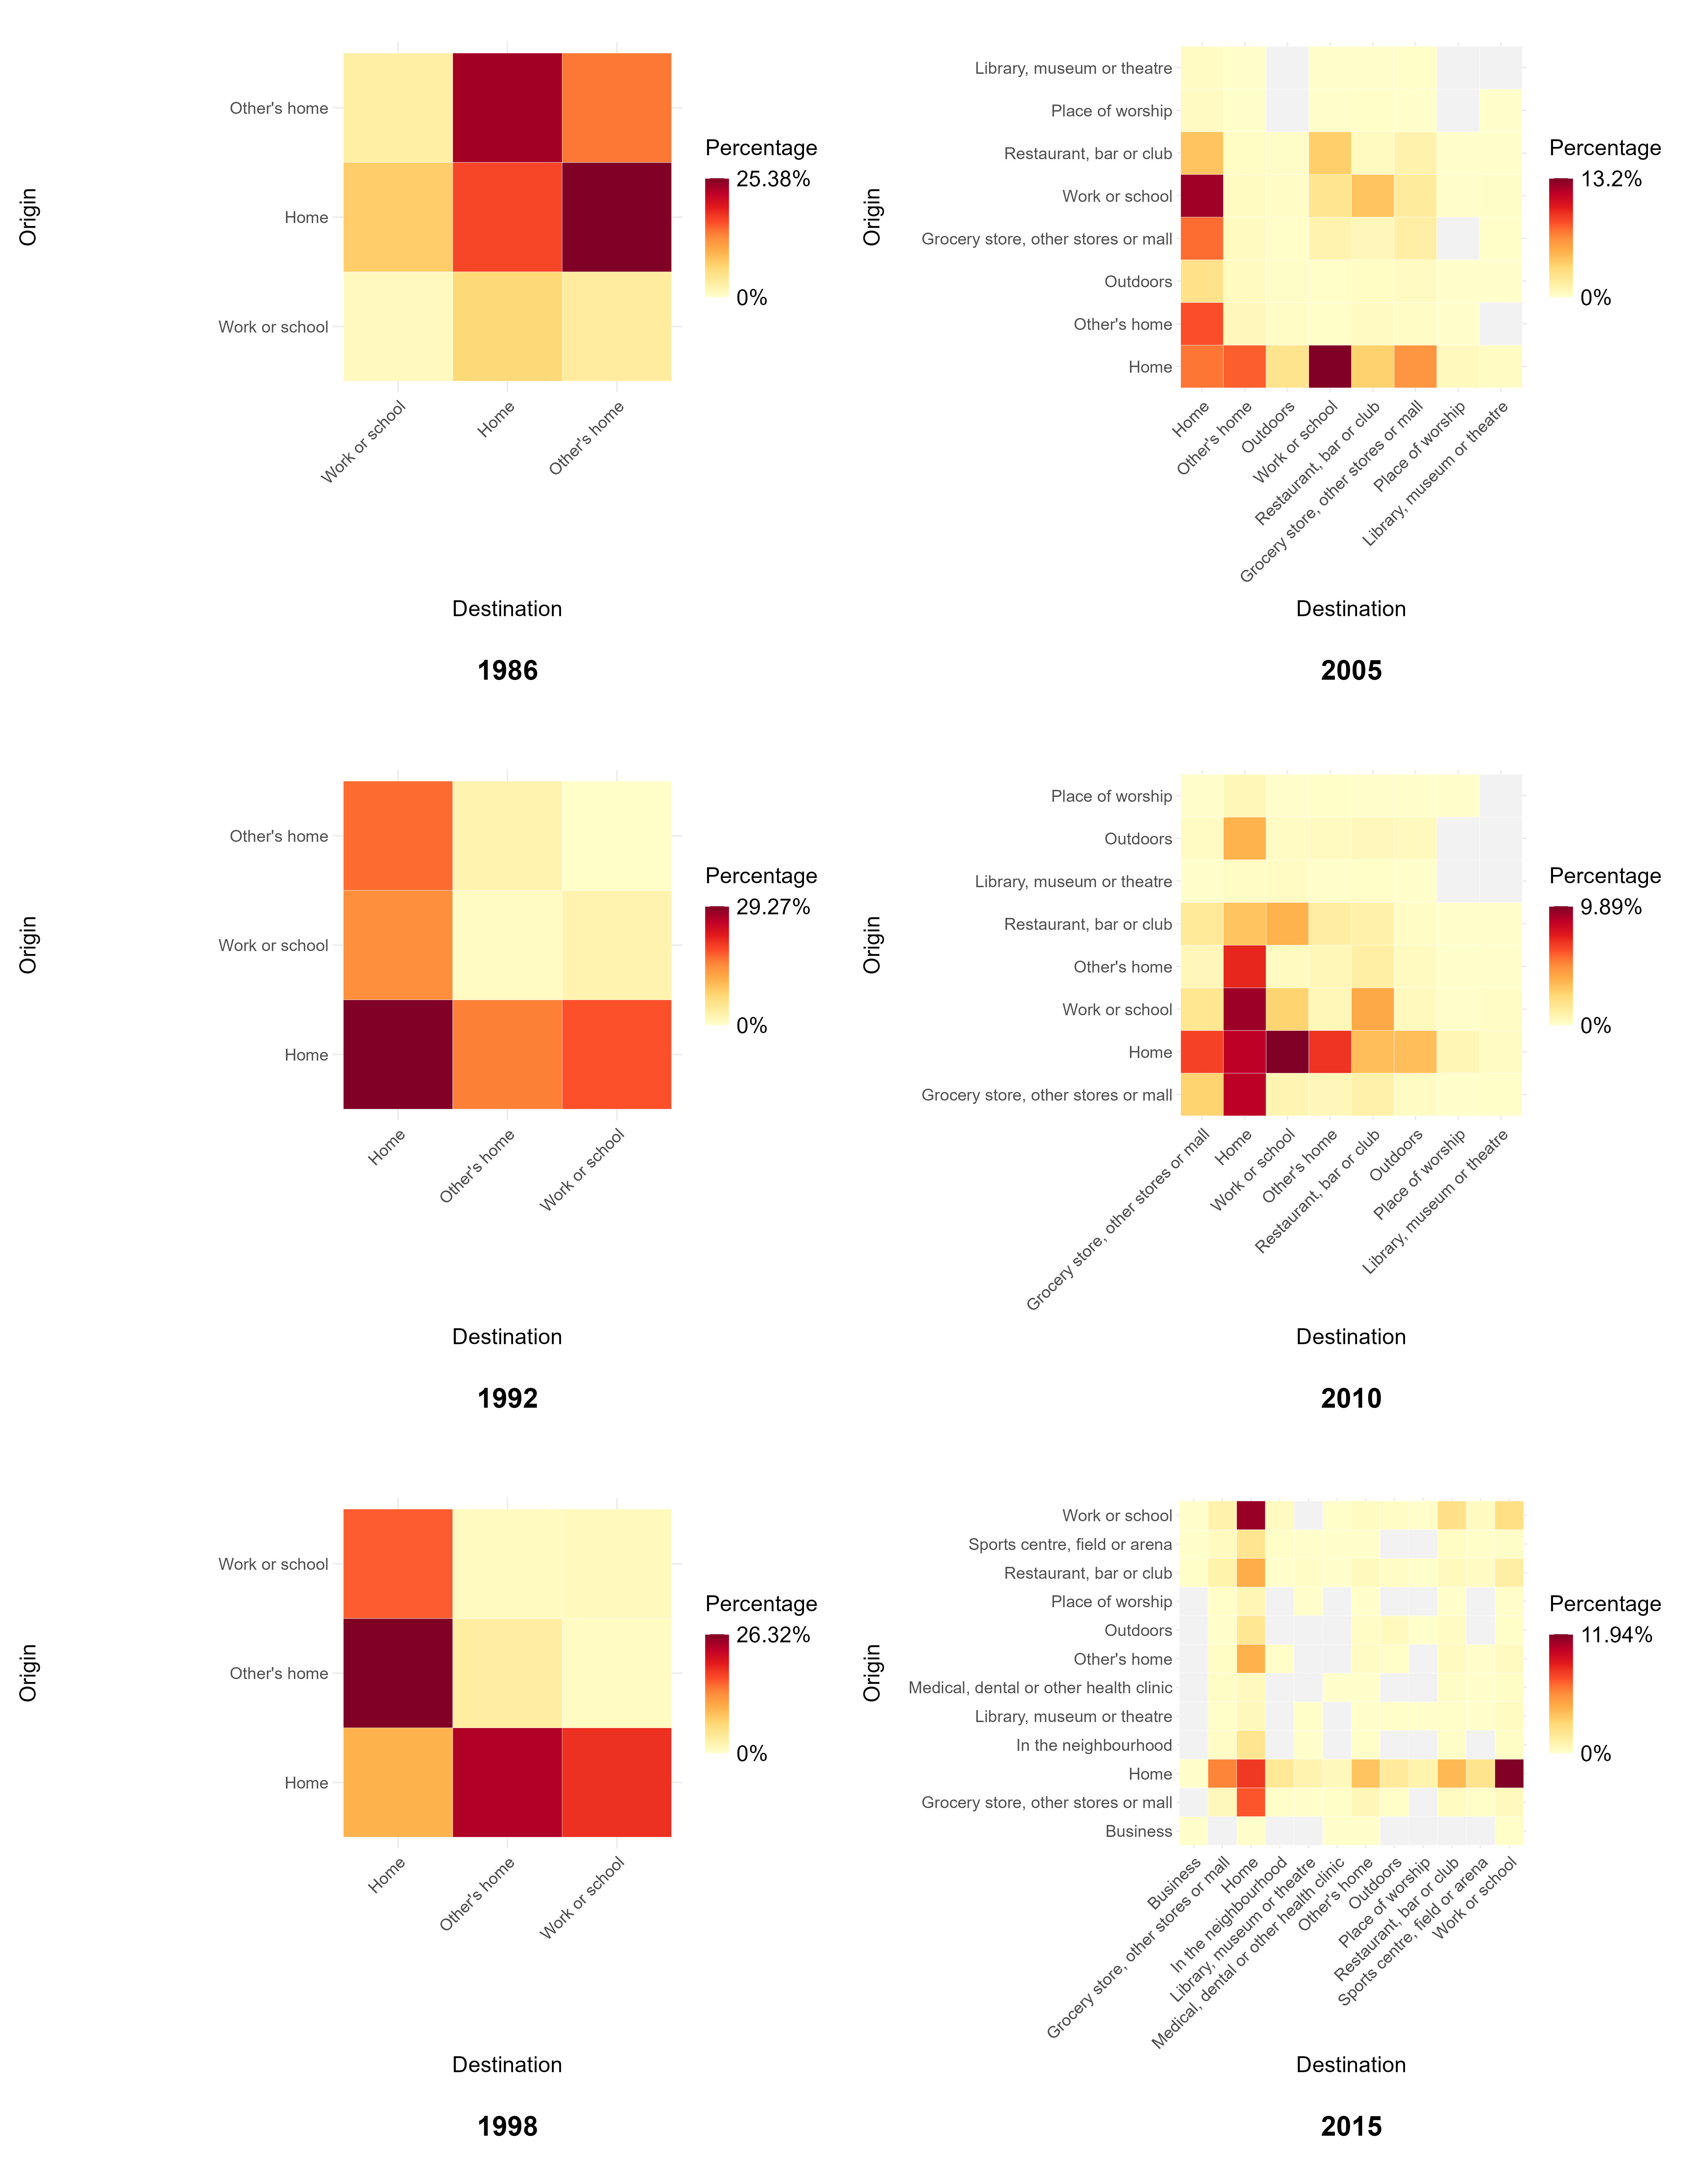
\includegraphics[width=1\linewidth]{figure/ch03_fig_01} 

}

\caption{Percentage of walking Trips Categorized by Origin and Destination}\label{fig:heat-w}
\end{figure}

In 2015, bicycles were clearly preferred as a primary mode of transportation, especially for commuting from `home' to `work or school,' accounting for 32.73\% of all cycling trips. It underscores the bicycle's role in daily commutes, reflecting a commitment to environmental sustainability and fitness. The return journey from work or school to home also showed a significant volume, representing 30.38\% of trips, indicating a balanced bidirectional commuting pattern. Besides commuting, cycling for errands and social visitations was notable, with trips to grocery stores and other retail destinations making up 5.41\% and trips for social purposes to another's home at 3.66\%. Leisure activities, including visits to restaurants, bars, or clubs, accounted for 2.06\% of trips. Additionally, trips from home to home were reported at 4.58\%, highlighting cycling's role in local mobility.

Commuting remained a key cycling activity in 2010, with 27.97\% of trips made from `home' to `work or school' and 25.38\% in the opposite direction, reinforcing the bicycle's importance in daily travel. Social interactions played a significant role, with 8.71\% of trips from `home' to `other's home' integrating bicycles into the social fabric of Canadian life. Errands and dining or entertainment purposes remained consistent with previous years, at 5.01\% and 2.06\%, respectively. Home-to-home trips accounted for 5.97\%, underscoring the versatility of cycling for various personal needs.

By 2005, the landscape of cycling trips showed a diverse usage pattern, with commuting still at 18.74\% for trips from `work or school' to `home'. The data highlights the bicycle's vital role in Canadian daily life as a reliable mode of transport. Interestingly, trips from `home' to `home' constituted 7.85\% of the total, indicating that a significant portion of cycling activity was dedicated to local and recreational mobility. Social and errand cycling, at 7.06\% and 7.15\%, respectively, along with recreational trips, at 2.07\%, show the broadening scope of cycling beyond mere commuting.

In 1998, the data presented a deep color saturation on the heat map for trips from `work or school' to `home' and vice versa, with 26.64\% and 30.75\% of trips, respectively, highlighting a strong bidirectional commuting behavior. The role of bicycles in social visitation was also significant, with 13.53\% of trips from `home' to `other's home' and 20.74\% for the return journey. Home-to-home trips were 4.18\%, pointing to the growing trend of using bicycles for a mix of commuting, social, and recreational purposes.The bicycle's essential role in commuting was further reinforced in 1992 when data showed that 26.13\% of cycling trips were made from ``home'' to ``work or school,'' with a sizable return trip percentage of 20.33\%. Social visitations also featured prominently, with 20.74\% of trips from `other's home' back to `home', indicating the bicycle's role in facilitating community connectivity. Cycling trips within the `home' category, indicating a variety of local uses, were at 15.03\%.

Over the years, the cycling trends in Canada have shown an evolving pattern, with a consistent emphasis on commuting while also demonstrating an increasing integration of bicycles into various aspects of urban life. In 2015, cycling was predominantly used for commuting, with 32.73\% of trips from `home' to `work or school' and a nearly equal percentage for the return journey. This trend reflects a strong environmental and fitness consciousness in urban Canadian society. Comparatively, in 2010, while commuting still remained the primary use of bicycles (27.97\% for going to work or school and 25.38\% for returning), there was a noticeable increase in cycling for social visitations, accounting for 8.71\% of trips. This shift indicates a broader adoption of cycling beyond utilitarian purposes, embedding it more deeply into the social fabric.

In earlier years, such as 2005 and 1998, the emphasis on commuting was still apparent but with a slightly different focus. For instance 2005, the most prevalent cycling route was from work or school to home, constituting 18.74\% of trips. This difference in the direction of the dominant route might suggest variations in cycling habits or available infrastructure at the time. In 1998, the data showed a balance between commuting and social interactions, with high percentages for trips from work or school to home (26.64\%) and from `home' to `other's home' (13.53\%). This balance demonstrates the role of bicycles in fostering community interactions and local mobility. Going back to 1992, cycling for commuting (26.13\%) and social visitations (20.74\%) were also significant, highlighting the bicycle's longstanding role in facilitating professional and interpersonal connectivity.

Overall, these trends across different years illustrate a consistent reliance on bicycles for commuting in Canada, coupled with a growing appreciation of their role in social and recreational activities. The shifting percentages and patterns of use reflect changing urban lifestyles, advancements in cycling infrastructure, and an increasing recognition of the bicycle as a versatile, environmentally friendly, and health-conscious mode of transportation in Canadian cities

\hypertarget{impedance-function-analysis}{%
\subsection{Impedance function analysis}\label{impedance-function-analysis}}

The impedance function figures presented in this section illuminate the changes in walking and cycling trip durations to various destinations across Canada over an extensive period from 1986 to 2015. These distance decay curves are pivotal to understanding impedance functions and are critical for travel behavior analysis. A fundamental idea of spatial interaction is represented by their depiction of the decreasing probability of selecting walking or cycling as a mode of transportation as the distance between the origin and the destination increases. This idea states that the likelihood of traveling between two points decreases with increasing distance. These curves also indicate the critical points at which a person's tendency to walk or cycle abruptly decreases.

Our exploration of distance decay curves for walking and cycling trips to diverse destinations utilized the General Social Survey (GSS) dataset, enabling an examination of how these curves vary across transportation modes and destination types over time. The data shed light on the frequency and characteristics of walking and cycling trips, with the years 2005, 2010, and 2015 featuring a wide range of destinations, from homes to workplaces, schools, other people's homes, grocery stores, retail outlets, malls, outdoor spaces, restaurants, bars, clubs, libraries, museums, theaters, and places of worship. This breadth of destination types signifies a marked expansion from the data of earlier years (1986, 1992, and 1998), which cataloged trips primarily to homes, other people's homes, and work or school. This evolution in data collection reflects a growing understanding of the complex nature of urban mobility and the diverse purposes that motivate walking and cycling trips, providing a comprehensive foundation for analyzing distance decay and its implications for urban planning and sustainable transportation strategies.

A methodical statistical approach was adopted to determine the appropriate distribution for modeling the distance decay curves for different destinations. The analysis began with generating Cullen and Frey graphs utilizing the fitdistrplus package in R, a graphical tool pivotal for suggesting plausible distributions by plotting the square of skewness against excess kurtosis. This step paved the way for selecting potential distributions for further assessment. Upon identifying potential distributions, an empirical evaluation was conducted to fit several candidate distributions to the data, specifically targeting distributions such as Gamma, Weibull, normal, lognormal, poisson, logistic, and Exponential, among others. Each distribution was fitted using maximum likelihood estimation (MLE), with the added complexity of weights incorporated into the fitting process. This was a crucial step as the dataset included a weight variable, which is a fundamental weighting element used for estimating the frequency of activities conducted by the Canadian population as recorded in the dataset. It aims to portray the broader behavioral patterns of the population accurately.

To objectively assess the fit of each distribution, model selection criteria such as the Akaike Information Criterion (AIC), Bayesian Information Criterion (BIC), and log-likelihood (logLik) were employed. These criteria are critical in not only capturing the goodness of fit but also penalizing the complexity of the model to prevent overfitting. AIC and BIC provide a balance between the model's accuracy and complexity, where lower values are indicative of a more economical model. The log-likelihood directly measures the probability of observing the given data under the assumed statistical model, with higher values signaling a better fit. The distribution that manifested the lowest AIC and BIC, coupled with the highest log-likelihood, was deemed the most suitable for representing the distance decay curve for each specific destination in each year. This rigorous statistical procedure ensured that the chosen distribution was the most fitting given the empirical data, reflecting both the underlying process and the observed variations. The approach guarantees that the final model is not only statistically robust but also reliable for interpreting the distance decay effect within the study context. Despite initial considerations for traditional diagnostic methods such as residual analysis and Q-Q plots, these techniques proved incompatible with the complexities of weighted data. The variable ``WGHT\_EPI'' in the dataset weighting variable is essential for representing the Canadian population's activity frequencies at the episode level. While the fitdistrplus package accommodates weights in estimation, it does not extend this functionality to diagnostic plots, which are typically unweighted. Consequently, the reliance on information criteria like AIC and BIC, adjusted for weighted data, became instrumental in guiding our selection of the most robust and representative model for our analysis, marking a methodological stride in our statistical practice.

Following the detailed statistical analysis, we present four comprehensive tables that encapsulate AIC, BIC, and log-likelihood values of each destination by mode and year (Tables \ref{tab:table_16},\ref{tab:table_17}, \ref{tab:table_18}, and \ref{tab:table_19}). These tables summarize the fitting process for each distribution evaluated, illuminating the decision-making process for selecting the most suitable distribution for each destination category. The tables illustrate our model selection process, highlighting the distribution that emerged as the best fit for each specific context based on the lowest AIC and BIC values and the highest log-likelihood scores. The first table delineates the statistical metrics for walking trips, while the second table deals with trips made by bicycle. Each table is organized to showcase the comparison across different years, thus offering insights into the temporal dynamics of travel behavior and the evolution of distance decay characteristics. By presenting the diagnostics in this tabular format, we aim to provide a clear and accessible reference demonstrating the distributional trends and patterns discerned from the GSS dataset.

\begin{table}
\centering
\caption{\label{tab:table-imw1}\label{tab:table_16}Impedance functions and selection criteria across different destinations for walking trips (1986, 1992 and 1998)}
\centering
\fontsize{9}{11}\selectfont
\begin{tabular}[t]{llrrr}
\toprule
Impedance\_Function & year & logLik & AIC & BIC\\
\midrule
\addlinespace[0.3em]
\multicolumn{5}{l}{\textbf{Destination: Home}}\\
\hspace{1em}Gamma & 1986 & -679.70 & 1363.40 & 1369.64\\
\hspace{1em}Weibull & 1986 & NA & NA & \vphantom{2} NA\\
\hspace{1em}Exponential & 1986 & -692.66 & 1387.32 & 1390.43\\
\hspace{1em}Gamma & 1992 & -3445.93 & 6895.85 & 6905.38\\
\hspace{1em}Weibull & 1992 & NA & NA & \vphantom{1} NA\\
\hspace{1em}Exponential & 1992 & -3462.38 & 6926.75 & 6931.52\\
\hspace{1em}Gamma & 1998 & -2822.99 & 5649.98 & 5659.47\\
\hspace{1em}Weibull & 1998 & NA & NA & \vphantom{1} NA\\
\hspace{1em}Exponential & 1998 & -2829.02 & 5660.04 & 5664.78\\
\addlinespace[0.3em]
\multicolumn{5}{l}{\textbf{Destination: Other's home}}\\
\hspace{1em}Gamma & 1986 & -646.37 & 1296.75 & 1302.91\\
\hspace{1em}Weibull & 1986 & NA & NA & \vphantom{1} NA\\
\hspace{1em}Exponential & 1986 & -655.12 & 1312.24 & 1315.32\\
\hspace{1em}Lognormal & 1986 & NA & NA & \vphantom{1} NA\\
\hspace{1em}Gamma & 1992 & -1097.09 & 2198.17 & 2205.70\\
\hspace{1em}Weibull & 1992 & -1108.03 & 2220.05 & 2227.58\\
\hspace{1em}Exponential & 1992 & -1114.47 & 2230.94 & 2234.70\\
\hspace{1em}Lognormal & 1992 & NA & NA & \vphantom{1} NA\\
\hspace{1em}Gamma & 1998 & -1493.73 & 2991.47 & 2999.76\\
\hspace{1em}Weibull & 1998 & -1498.74 & 3001.47 & 3009.77\\
\hspace{1em}Exponential & 1998 & -1499.40 & 3000.80 & 3004.95\\
\hspace{1em}Lognormal & 1998 & NA & NA & \vphantom{1} NA\\
\addlinespace[0.3em]
\multicolumn{5}{l}{\textbf{Destination: Work or school}}\\
\hspace{1em}Gamma & 1986 & -243.98 & 491.96 & 496.01\\
\hspace{1em}Weibull & 1986 & NA & NA & NA\\
\hspace{1em}Exponential & 1986 & -246.96 & 495.93 & 497.96\\
\hspace{1em}Lognormal & 1986 & NA & NA & NA\\
\hspace{1em}Gamma & 1992 & -976.83 & 1957.66 & 1964.99\\
\hspace{1em}Weibull & 1992 & NA & NA & NA\\
\hspace{1em}Exponential & 1992 & -1021.74 & 2045.48 & 2049.14\\
\hspace{1em}Lognormal & 1992 & NA & NA & NA\\
\hspace{1em}Gamma & 1998 & -1173.77 & 2351.53 & 2359.19\\
\hspace{1em}Weibull & 1998 & NA & NA & NA\\
\hspace{1em}Exponential & 1998 & -1177.45 & 2356.91 & 2360.74\\
\hspace{1em}Lognormal & 1998 & NA & NA & NA\\
\bottomrule
\end{tabular}
\end{table}

The figures below illustrate the frequency distribution of travel times for walking and cycling to various destinations, as modeled by impedance functions over a range of years. Each graph shows a curve representing the scaled frequency of trips against the trip duration in minutes for a specific year, with the peak of the curve indicating the most common trip duration. The red dots and dashed lines highlight the mode of the distribution, which is the most frequently observed trip duration. The multiple curves within each year show the variability or sensitivity of the model under different assumptions or parameters.
From these figures, we can infer trends in travel behavior for walking and cycling over time. For instance, a shift in the peak towards the right over the years would suggest an increase in the average duration of trips, possibly due to several factors such as urban sprawl, changes in urban design, or evolving societal preferences. Conversely, a shift towards the left would suggest a decrease in trip duration, potentially indicating improved walking and cycling infrastructure, leading to shorter and possibly more convenient trips.
These figures encapsulate a wealth of information about travel behavior and serve as a visual summary of the underlying data collected for walking and cycling trips to different destinations. They provide a snapshot of the changes in travel time preferences or requirements across the studied years, which is valuable for urban planners and policymakers aiming to understand and promote sustainable modes of transportation.

\hypertarget{conclusion}{%
\chapter*{Conclusion}\label{conclusion}}
\addcontentsline{toc}{chapter}{Conclusion}

This study has embarked on a comprehensive journey through three decades of active travel behavior in Canada, from 1986 to 2015, leveraging data from the General Social Survey (GSS) to shed light on individual preferences and behaviors regarding walking and cycling. This exploration is particularly relevant as it spans a period of significant urban development, evolving societal attitudes towards health and the environment, and transformations in transportation infrastructure and policies.
Our results show that walking and cycling have consistently longer trip times, with shorter walking trips. Between 1986 and 2005, this gap shrunk, suggesting the intricate interactions between urban sprawl, a greater reliance on motorized transportation, and shifting preferences.git pus From 2005 to 2015, walking and cycling trip durations increased, likely influenced by heightened urbanization, health and sustainability concerns awareness, and urban planning shifts towards active transportation.

The study also uncovered trends in trip destinations, with cycling trips in 2015 primarily directed towards homes, schools, and workplaces, highlighting cycling's emergence as a sustainable commuting option. Walking trips predominantly originated from residential areas to workplaces and educational institutions, reflecting a shift towards walking for eco-friendly and health-conscious commuting.
However, the research encountered limitations, notably in handling weighted data for statistical tests and model diagnostics. The reliance on AIC, BIC, and log-likelihood values underscores the necessity for advanced tools that accommodate weighted data, addressing a methodological gap in statistical practices. The absence of cycling data further limits our analysis, presenting an avenue for future research to explore cycling trends and its potential as an alternative transportation mode for accessing cultural venues.

In light of these limitations, future research should prioritize the development of methodologies and diagnostic tools that effectively incorporate weighted data, enhancing the robustness and representativeness of findings in survey-based analyses. Investigating cycling data could also provide a fuller picture of active travel behaviors and their implications for urban planning and policy-making.
In conclusion, this thesis presents a detailed account of the evolution of active travel behaviors in Canada over three decades, highlighting the resurgence of walking and cycling as key modes of transportation. These insights are invaluable for urban planners, policymakers, and researchers striving to foster sustainable and active transportation systems. Future research can further enrich our understanding of active travel behaviors and support efforts to promote sustainable mobility options by addressing the identified methodological challenges and exploring underrepresented areas such as cycling trends.

\hypertarget{references}{%
\chapter*{References}\label{references}}
\addcontentsline{toc}{chapter}{References}

Placeholder

\hypertarget{refs}{}
\begin{CSLReferences}{1}{0}
\leavevmode\vadjust pre{\hypertarget{ref-apparicio2008comparing}{}}%
Apparicio, P., Abdelmajid, M., Riva, M., \& Shearmur, R. (2008). Comparing alternative approaches to measuring the geographical accessibility of urban health services: Distance types and aggregation-error issues. \emph{International Journal of Health Geographics}, \emph{7}(1), 1--14.

\leavevmode\vadjust pre{\hypertarget{ref-arranz2019measuring}{}}%
Arranz-Lopez, A., Soria-Lara, J. A., Witlox, F., \& Paez, A. (2019). Measuring relative non-motorized accessibility to retail activities. \emph{International Journal of Sustainable Transportation}, \emph{13}(9), 639--651.

\leavevmode\vadjust pre{\hypertarget{ref-bhat2002development}{}}%
Bhat, C., Handy, S., Kockelman, K., Mahmassani, H., Gopal, A., Srour, I., \& Weston, L. (2002). Development of an urban accessibility index: Formulations, aggregation, and application. \emph{Work}, \emph{4938}(4).

\leavevmode\vadjust pre{\hypertarget{ref-breheny1978measurement}{}}%
Breheny, M. J. (1978). The measurement of spatial opportunity in strategic planning. \emph{Regional Studies}, \emph{12}(4), 463--479.

\leavevmode\vadjust pre{\hypertarget{ref-carrothers1956historical}{}}%
Carrothers, G. A. (1956). An historical review of the gravity and potential concepts of human interaction. \emph{Journal of the American Institute of Planners}, \emph{22}(2), 94--102.

\leavevmode\vadjust pre{\hypertarget{ref-cascetta2013new}{}}%
Cascetta, E., Carteni, A., \& Montanino, M. (2013). A new measure of accessibility based on perceived opportunities. \emph{Procedia-Social and Behavioral Sciences}, \emph{87}, 117--132.

\leavevmode\vadjust pre{\hypertarget{ref-church2003measuring}{}}%
Church, R. L., \& Marston, J. R. (2003). Measuring accessibility for people with a disability. \emph{Geographical Analysis}, \emph{35}(1), 83--96.

\leavevmode\vadjust pre{\hypertarget{ref-clifton2001evaluating}{}}%
Clifton, K. J., \& Handy, S. (2001). Evaluating neighborhood accessibility: Possibilities and practicalities. \emph{Journal of Transportation and Statistics}, \emph{4}(2-3), 67.

\leavevmode\vadjust pre{\hypertarget{ref-currie2010quantifying}{}}%
Currie, G. (2010). Quantifying spatial gaps in public transport supply based on social needs. \emph{Journal of Transport Geography}, \emph{18}(1), 31--41.

\leavevmode\vadjust pre{\hypertarget{ref-de2009exponential}{}}%
De Vries, J. J., Nijkamp, P., \& Rietveld, P. (2009). Exponential or power distance-decay for commuting? An alternative specification. \emph{Environment and Planning A}, \emph{41}(2), 461--480.

\leavevmode\vadjust pre{\hypertarget{ref-delignette2015fitdistrplus}{}}%
Delignette-Muller, M. L., \& Dutang, C. (2015). Fitdistrplus: An r package for fitting distributions. \emph{Journal of Statistical Software}, \emph{64}, 1--34.

\leavevmode\vadjust pre{\hypertarget{ref-de2011modelling}{}}%
Dios Ortuzar, J. de, \& Willumsen, L. G. (2011). \emph{Modelling transport}. John wiley \& sons.

\leavevmode\vadjust pre{\hypertarget{ref-eldridge1991warped}{}}%
Eldridge, J. D., \& Jones III, J. P. (1991). Warped space: A geography of distance decay. \emph{The Professional Geographer}, \emph{43}(4), 500--511.

\leavevmode\vadjust pre{\hypertarget{ref-fotheringham1981spatial}{}}%
Fotheringham, A. S. (1981). Spatial structure and distance-decay parameters. \emph{Annals of the Association of American Geographers}, \emph{71}(3), 425--436.

\leavevmode\vadjust pre{\hypertarget{ref-fotheringham1989spatial}{}}%
Fotheringham, A. S., \& O'Kelly, M. E. (1989). \emph{Spatial interaction models: Formulations and applications} (Vol. 1). Kluwer Academic Publishers Dordrecht.

\leavevmode\vadjust pre{\hypertarget{ref-frank2001built}{}}%
Frank, L. D., \& Engelke, P. O. (2001). The built environment and human activity patterns: Exploring the impacts of urban form on public health. \emph{Journal of Planning Literature}, \emph{16}(2), 202--218.

\leavevmode\vadjust pre{\hypertarget{ref-frank2005linking}{}}%
Frank, L. D., Schmid, T. L., Sallis, J. F., Chapman, J., \& Saelens, B. E. (2005). Linking objectively measured physical activity with objectively measured urban form: Findings from SMARTRAQ. \emph{American Journal of Preventive Medicine}, \emph{28}(2), 117--125.

\leavevmode\vadjust pre{\hypertarget{ref-gaudry1981inverse}{}}%
Gaudry, M. J. (1981). The inverse power transformation logit and dogit mode choice models. \emph{Transportation Research Part B: Methodological}, \emph{15}(2), 97--103.

\leavevmode\vadjust pre{\hypertarget{ref-geertman1995gis}{}}%
Geertman, S. C., \& Ritsema Van Eck, J. R. (1995). GIS and models of accessibility potential: An application in planning. \emph{International Journal of Geographical Information Systems}, \emph{9}(1), 67--80.

\leavevmode\vadjust pre{\hypertarget{ref-geurs2006accessibility}{}}%
Geurs, K. (2006). \emph{Accessibility, land use and transport: Accessibility evaluation of land-use and transport developments and policy strategy}. Eburon Uitgeverij BV.

\leavevmode\vadjust pre{\hypertarget{ref-geurs2001accessibility}{}}%
Geurs, K. T., \& Ritsema van Eck, J. R. (2001). Accessibility measures: Review and applications. Evaluation of accessibility impacts of land-use transportation scenarios, and related social and economic impact. \emph{RIVM Rapport 408505006}.

\leavevmode\vadjust pre{\hypertarget{ref-geurs2004}{}}%
Geurs, K. T., \& Van Wee, B. (2004). Accessibility evaluation of land-use and transport strategies: Review and research directions. \emph{Journal of Transport Geography}, \emph{12}(2), 127--140.

\leavevmode\vadjust pre{\hypertarget{ref-grengs2004measuring}{}}%
Grengs, J. (2004). Measuring change in small-scale transit accessibility with geographic information systems: Buffalo and rochester, new york. \emph{Transportation Research Record}, \emph{1887}(1), 10--17.

\leavevmode\vadjust pre{\hypertarget{ref-grengs2015nonwork}{}}%
Grengs, J. (2015). Nonwork accessibility as a social equity indicator. \emph{International Journal of Sustainable Transportation}, \emph{9}(1), 1--14.

\leavevmode\vadjust pre{\hypertarget{ref-gutierrez1996european}{}}%
Gutierrez, J., Gonzalez, R., \& Gomez, G. (1996). The european high-speed train network: Predicted effects on accessibility patterns. \emph{Journal of Transport Geography}, \emph{4}(4), 227--238.

\leavevmode\vadjust pre{\hypertarget{ref-haggett2001geography}{}}%
Haggett, P. (2001). \emph{Geography: A global synthesis}. Pearson Education.

\leavevmode\vadjust pre{\hypertarget{ref-halas2014distance}{}}%
Halas, M., Klapka, P., \& Kladivo, P. (2014). Distance-decay functions for daily travel-to-work flows. \emph{Journal of Transport Geography}, \emph{35}, 107--119.

\leavevmode\vadjust pre{\hypertarget{ref-hamidi2014applying}{}}%
Hamidi, Z. (2014). \emph{Applying accessibility measures to explore the integration of bicycle and transmilenio system in the city of bogota} (Master's thesis). University of Twente.

\leavevmode\vadjust pre{\hypertarget{ref-handy1993regional}{}}%
Handy, S. (1993). Regional versus local accessibility: Implications for nonwork travel.

\leavevmode\vadjust pre{\hypertarget{ref-handy1997measuring}{}}%
Handy, S. L., \& Niemeier, D. A. (1997). Measuring accessibility: An exploration of issues and alternatives. \emph{Environment and Planning A}, \emph{29}(7), 1175--1194.

\leavevmode\vadjust pre{\hypertarget{ref-hansen1959accessibility}{}}%
Hansen, W. G. (1959). How accessibility shapes land use. \emph{Journal of the American Institute of Planners}, \emph{25}(2), 73--76.

\leavevmode\vadjust pre{\hypertarget{ref-hess2005access}{}}%
Hess, D. B. (2005). Access to employment for adults in poverty in the buffalo-niagara region. \emph{Urban Studies}, \emph{42}(7), 1177--1200.

\leavevmode\vadjust pre{\hypertarget{ref-hino2014built}{}}%
Hino, A. A., Reis, R. S., Sarmiento, O. L., Parra, D. C., \& Brownson, R. C. (2014). Built environment and physical activity for transportation in adults from curitiba, brazil. \emph{Journal of Urban Health}, \emph{91}, 446--462.

\leavevmode\vadjust pre{\hypertarget{ref-hsiao1997use}{}}%
Hsiao, S., Lu, J., Sterling, J., \& Weatherford, M. (1997). Use of geographic information system for analysis of transit pedestrian access. \emph{Transportation Research Record}, \emph{1604}(1), 50--59.

\leavevmode\vadjust pre{\hypertarget{ref-hull2012accessibility}{}}%
Hull, A., Silva, C., \& Bertolini, L. (2012). \emph{Accessibility instruments for planning practice}. Cost Office Brussels.

\leavevmode\vadjust pre{\hypertarget{ref-iacono2010}{}}%
Iacono, M., Krizek, K. J., \& El-Geneidy, A. (2010). Measuring non-motorized accessibility: Issues, alternatives, and execution. \emph{Journal of Transport Geography}, \emph{18}(1), 133--140.

\leavevmode\vadjust pre{\hypertarget{ref-iacono2008access}{}}%
Iacono, M., Krizek, K., \& El-Geneidy, A. M. (2008). Access to destinations: How close is close enough? Estimating accurate distance decay functions for multiple modes and different purposes.

\leavevmode\vadjust pre{\hypertarget{ref-ingram1971concept}{}}%
Ingram, D. R. (1971). The concept of accessibility: A search for an operational form. \emph{Regional Studies}, \emph{5}(2), 101--107.

\leavevmode\vadjust pre{\hypertarget{ref-itf2017linking}{}}%
ITF. (2017). \emph{Linking people and places: New ways of understanding spatial access in cities}. OECD Publishing.

\leavevmode\vadjust pre{\hypertarget{ref-johnston1973frictions}{}}%
Johnston, R. J. (1973). On frictions of distance and regression coefficients. \emph{Area}, 187--191.

\leavevmode\vadjust pre{\hypertarget{ref-kanafani1983transportation}{}}%
Kanafani, A. (1983). Transportation demand analysis.

\leavevmode\vadjust pre{\hypertarget{ref-koenig1980indicators}{}}%
Koenig, J.-G. (1980). Indicators of urban accessibility: Theory and application. \emph{Transportation}, \emph{9}(2), 145--172.

\leavevmode\vadjust pre{\hypertarget{ref-krizek2005perspectives}{}}%
Krizek, K. J. (2005). Perspectives on accessibility and travel. In \emph{Access to destinations} (pp. 109--130). Emerald Group Publishing Limited.

\leavevmode\vadjust pre{\hypertarget{ref-kwan1998space}{}}%
Kwan, M.-P. (1998). Space-time and integral measures of individual accessibility: A comparative analysis using a point-based framework. \emph{Geographical Analysis}, \emph{30}(3), 191--216.

\leavevmode\vadjust pre{\hypertarget{ref-kwan2003recent}{}}%
Kwan, M.-P., Murray, A. T., OKelly, M. E., \& Tiefelsdorf, M. (2003). Recent advances in accessibility research: Representation, methodology and applications. \emph{Journal of Geographical Systems}, \emph{5}, 129--138.

\leavevmode\vadjust pre{\hypertarget{ref-lamiquiz2015effects}{}}%
Lamiquiz, P. J., \& Lopez-Dominguez, J. (2015). Effects of built environment on walking at the neighbourhood scale. A new role for street networks by modelling their configurational accessibility? \emph{Transportation Research Part A: Policy and Practice}, \emph{74}, 148--163.

\leavevmode\vadjust pre{\hypertarget{ref-larsen2010beyond}{}}%
Larsen, J., El-Geneidy, A., \& Yasmin, F. (2010). Beyond the quarter mile: Re-examining travel distances by active transportation. \emph{Canadian Journal of Urban Research}, \emph{19}(1), 70--88.

\leavevmode\vadjust pre{\hypertarget{ref-levinson2005access}{}}%
Levinson, D. M., \& Krizek, K. J. (2005). \emph{Access to destinations}. Elsevier Publishers.

\leavevmode\vadjust pre{\hypertarget{ref-li2020approach}{}}%
Li, A., Huang, Y., \& Axhausen, K. W. (2020). An approach to imputing destination activities for inclusion in measures of bicycle accessibility. \emph{Journal of Transport Geography}, \emph{82}, 102566.

\leavevmode\vadjust pre{\hypertarget{ref-lowry2012using}{}}%
Lowry, M., Callister, D., Gresham, M., \& Moore, B. (2012). Using bicycle level of service to assess community-wide bikeability. In \emph{91st annual meeting of the transportation research board, washington, DC: Transportation research board}.

\leavevmode\vadjust pre{\hypertarget{ref-luoma1993threshold}{}}%
Luoma, M., Mikkonen, K., \& Palomaki, M. (1993). The threshold gravity model and transport geography: How transport development influences the distance-decay parameter of the gravity model. \emph{Journal of Transport Geography}, \emph{1}(4), 240--247.

\leavevmode\vadjust pre{\hypertarget{ref-mandel1997disaggregate}{}}%
Mandel, B., Gaudry, M., \& Rothengatter, W. (1997). A disaggregate box-cox logit mode choice model of intercity passenger travel in germany and its implications for high-speed rail demand forecasts. \emph{The Annals of Regional Science}, \emph{31}, 99--120.

\leavevmode\vadjust pre{\hypertarget{ref-martinez2013new}{}}%
Martinez, L. M., \& Viegas, J. M. (2013). A new approach to modelling distance-decay functions for accessibility assessment in transport studies. \emph{Journal of Transport Geography}, \emph{26}, 87--96.

\leavevmode\vadjust pre{\hypertarget{ref-meyer1984urban}{}}%
Meyer, M. D., \& Miller, E. J. (1984). Urban transportation planning: A decision-oriented approach.

\leavevmode\vadjust pre{\hypertarget{ref-mikkonen1999parameters}{}}%
Mikkonen, K., \& Luoma, M. (1999). The parameters of the gravity model are changing--how and why? \emph{Journal of Transport Geography}, \emph{7}(4), 277--283.

\leavevmode\vadjust pre{\hypertarget{ref-miller2005place}{}}%
Miller, H. J. (2005). Place-based versus people-based accessibility. In \emph{Access to destinations} (pp. 63--89). Emerald Group Publishing Limited.

\leavevmode\vadjust pre{\hypertarget{ref-millward2013active}{}}%
Millward, H., Spinney, J., \& Scott, D. (2013). Active-transport walking behavior: Destinations, durations, distances. \emph{Journal of Transport Geography}, \emph{28}, 101--110.

\leavevmode\vadjust pre{\hypertarget{ref-mozolin2000trip}{}}%
Mozolin, M., Thill, J.-C., \& Usery, E. L. (2000). Trip distribution forecasting with multilayer perceptron neural networks: A critical evaluation. \emph{Transportation Research Part B: Methodological}, \emph{34}(1), 53--73.

\leavevmode\vadjust pre{\hypertarget{ref-nassir2016utility}{}}%
Nassir, N., Hickman, M., Malekzadeh, A., \& Irannezhad, E. (2016). A utility-based travel impedance measure for public transit network accessibility. \emph{Transportation Research Part A: Policy and Practice}, \emph{88}, 26--39.

\leavevmode\vadjust pre{\hypertarget{ref-osth2016new}{}}%
Osth, J., Lyhagen, J., \& Reggiani, A. (2016). A new way of determining distance decay parameters in spatial interaction models with application to job accessibility analysis in sweden. \emph{European Journal of Transport and Infrastructure Research}, \emph{16}(2).

\leavevmode\vadjust pre{\hypertarget{ref-paez2012measuring}{}}%
Paez, A., Scott, D. M., \& Morency, C. (2012). Measuring accessibility: Positive and normative implementations of various accessibility indicators. \emph{Journal of Transport Geography}, \emph{25}, 141--153.

\leavevmode\vadjust pre{\hypertarget{ref-papa2012gravity}{}}%
Papa, E., \& Coppola, P. (2012). Gravity-based accessibility measures for integrated transport-land use planning (GraBAM). \emph{Accessibility Instruments for Planning Practice}, \emph{117}, 124.

\leavevmode\vadjust pre{\hypertarget{ref-pirie1979measuring}{}}%
Pirie, G. H. (1979). Measuring accessibility: A review and proposal. \emph{Environment and Planning A}, \emph{11}(3), 299--312.

\leavevmode\vadjust pre{\hypertarget{ref-prins2014many}{}}%
Prins, R. G., Pierik, F., Etman, A., Sterkenburg, R. P., Kamphuis, C. B., \& Van Lenthe, F. (2014). How many walking and cycling trips made by elderly are beyond commonly used buffer sizes: Results from a GPS study. \emph{Health \& Place}, \emph{27}, 127--133.

\leavevmode\vadjust pre{\hypertarget{ref-reggiani2011accessibility}{}}%
Reggiani, A., Bucci, P., \& Russo, G. (2011). Accessibility and impedance forms: Empirical applications to the german commuting network. \emph{International Regional Science Review}, \emph{34}(2), 230--252.

\leavevmode\vadjust pre{\hypertarget{ref-richardson1969elements}{}}%
Richardson, H. W. et al. (1969). Elements of regional economics. \emph{Elements of Regional Economics.}

\leavevmode\vadjust pre{\hypertarget{ref-robinsonm}{}}%
Robinson, G. (n.d.). M., 1998: Methods and techniques in human geography. New York: Wiley \& Sons.

\leavevmode\vadjust pre{\hypertarget{ref-saghapour2017measuring}{}}%
Saghapour, T., Moridpour, S., \& Thompson, R. G. (2017). Measuring cycling accessibility in metropolitan areas. \emph{International Journal of Sustainable Transportation}, \emph{11}(5), 381--394.

\leavevmode\vadjust pre{\hypertarget{ref-sallis2004active}{}}%
Sallis, J. F., Frank, L. D., Saelens, B. E., \& Kraft, M. K. (2004). Active transportation and physical activity: Opportunities for collaboration on transportation and public health research. \emph{Transportation Research Part A: Policy and Practice}, \emph{38}(4), 249--268.

\leavevmode\vadjust pre{\hypertarget{ref-sen2012gravity}{}}%
Sen, A., \& Smith, T. E. (2012). \emph{Gravity models of spatial interaction behavior}. Springer Science \& Business Media.

\leavevmode\vadjust pre{\hypertarget{ref-signorino2011gravity}{}}%
Signorino, G., Pasetto, R., Gatto, E., Mucciardi, M., La Rocca, M., \& Mudu, P. (2011). Gravity models to classify commuting vs. Resident workers. An application to the analysis of residential risk in a contaminated area. \emph{International Journal of Health Geographics}, \emph{10}(1), 1--10.

\leavevmode\vadjust pre{\hypertarget{ref-skov2001estimation}{}}%
Skov-Petersen, H. (2001). Estimation of distance-decay parameters: GIS-based indicators of recreational accessibility. In \emph{ScanGIS} (pp. 237--258).

\leavevmode\vadjust pre{\hypertarget{ref-song1996some}{}}%
Song, S. (1996). Some tests of alternative accessibility measures: A population density approach. \emph{Land Economics}, 474--482.

\leavevmode\vadjust pre{\hypertarget{ref-stewart1941inverse}{}}%
Stewart, J. Q. (1941). An inverse distance variation for certain social influences. \emph{Science}, \emph{93}(2404), 89--90.

\leavevmode\vadjust pre{\hypertarget{ref-stewart1948demographic}{}}%
Stewart, J. Q. (1948). Demographic gravitation: Evidence and applications. \emph{Sociometry}, \emph{11}(1/2), 31--58.

\leavevmode\vadjust pre{\hypertarget{ref-sun2012measuring}{}}%
Sun, G., Lin, H., \& Li, R. (2012). Measuring the influence of built environment on walking behavior: An accessibility approach. In \emph{Geographic information science: 7th international conference, GIScience 2012, columbus, OH, USA, september 18-21, 2012. Proceedings 7} (pp. 187--197). Springer.

\leavevmode\vadjust pre{\hypertarget{ref-talen1998assessing}{}}%
Talen, E., \& Anselin, L. (1998). Assessing spatial equity: An evaluation of measures of accessibility to public playgrounds. \emph{Environment and Planning A}, \emph{30}(4), 595--613.

\leavevmode\vadjust pre{\hypertarget{ref-taylor1975distance}{}}%
Taylor, Peter. (1975). Distance decay models in spatial interactions. \emph{(No Title)}.

\leavevmode\vadjust pre{\hypertarget{ref-taylor1983distance}{}}%
Taylor, PJ. (1983). Distance decay in spatial interactions. CATMOG 2. Geo Books, Norwich.

\leavevmode\vadjust pre{\hypertarget{ref-taylor1971distance}{}}%
Taylor, P. J. (1971). Distance transformation and distance decay functions. \emph{Geographical Analysis}, \emph{3}(3), 221--238.

\leavevmode\vadjust pre{\hypertarget{ref-thorsen1999network}{}}%
Thorsen, I., Uboe, J., \& Naelig; vdal, G. (1999). A network approach to commuting. \emph{Journal of Regional Science}, \emph{39}(1), 73--101.

\leavevmode\vadjust pre{\hypertarget{ref-tiefelsdorf2003misspecifications}{}}%
Tiefelsdorf, M. (2003). Misspecifications in interaction model distance decay relations: A spatial structure effect. \emph{Journal of Geographical Systems}, \emph{5}, 25--50.

\leavevmode\vadjust pre{\hypertarget{ref-untermann1984accommodating}{}}%
Untermann, R. K. (1984). Accommodating the pedestrian: Adapting towns and neighbourhoods for walking and bicycling.

\leavevmode\vadjust pre{\hypertarget{ref-vale2017influence}{}}%
Vale, D. S., \& Pereira, M. (2017). The influence of the impedance function on gravity-based pedestrian accessibility measures: A comparative analysis. \emph{Environment and Planning B: Urban Analytics and City Science}, \emph{44}(4), 740--763.

\leavevmode\vadjust pre{\hypertarget{ref-van2001accessibility}{}}%
Van Wee, B., Hagoort, M., \& Annema, J. A. (2001). Accessibility measures with competition. \emph{Journal of Transport Geography}, \emph{9}(3), 199--208.

\leavevmode\vadjust pre{\hypertarget{ref-vandenbulcke2009mapping}{}}%
Vandenbulcke, G., Steenberghen, T., \& Thomas, I. (2009). Mapping accessibility in belgium: A tool for land-use and transport planning? \emph{Journal of Transport Geography}, \emph{17}(1), 39--53.

\leavevmode\vadjust pre{\hypertarget{ref-vasconcelos2012evaluation}{}}%
Vasconcelos, A. S., \& Farias, T. L. (2012). Evaluation of urban accessibility indicators based on internal and external environmental costs. \emph{Transportation Research Part D: Transport and Environment}, \emph{17}(6), 433--441.

\leavevmode\vadjust pre{\hypertarget{ref-vega2012using}{}}%
Vega, A. (2012). Using place rank to measure sustainable accessibility. \emph{Journal of Transport Geography}, \emph{24}, 411--418.

\leavevmode\vadjust pre{\hypertarget{ref-vickerman1974accessibility}{}}%
Vickerman, R. W. (1974). Accessibility, attraction, and potential: A review of some concepts and their use in determining mobility. \emph{Environment and Planning A}, \emph{6}(6), 675--691.

\leavevmode\vadjust pre{\hypertarget{ref-wilson1971family}{}}%
Wilson, A. G. (1971). A family of spatial interaction models, and associated developments. \emph{Environment and Planning A}, \emph{3}(1), 1--32.

\leavevmode\vadjust pre{\hypertarget{ref-wu2019measuring}{}}%
Wu, X., Lu, Y., Lin, Y., \& Yang, Y. (2019). Measuring the destination accessibility of cycling transfer trips in metro station areas: A big data approach. \emph{International Journal of Environmental Research and Public Health}, \emph{16}(15), 2641.

\leavevmode\vadjust pre{\hypertarget{ref-yang2012walking}{}}%
Yang, Y., \& Diez-Roux, A. V. (2012). Walking distance by trip purpose and population subgroups. \emph{American Journal of Preventive Medicine}, \emph{43}(1), 11--19.

\leavevmode\vadjust pre{\hypertarget{ref-zhao2003forecasting}{}}%
Zhao, F., Chow, L.-F., Li, M.-T., Ubaka, I., \& Gan, A. (2003). Forecasting transit walk accessibility: Regression model alternative to buffer method. \emph{Transportation Research Record}, \emph{1835}(1), 34--41.

\leavevmode\vadjust pre{\hypertarget{ref-zipf1949human}{}}%
Zipf, G. K. (1949). Human behavior and the principle of least effort: An introduction to human eoclogy.

\end{CSLReferences}

\end{document}
